%************************************************
\chapter{Development}
\label{ch:Development}
%************************************************

This chapter details the development phases of the battery health prediction system, covering the complete progress from initial MATLAB modeling to advanced deep learning implementation. The project evolved through distinct phases: (1) MATLAB-based modeling and simulation using traditional methods, (2) exploration of hybrid neural network approaches, (3) transition to pure data-driven models, and (4) implementation of state-of-the-art deep learning architectures for time series forecasting.

The development process was guided by the need to create accurate, strong, and scalable battery health prediction models capable of handling real world applications. Each phase built upon lessons learned from previous approaches, ultimately leading to the implementation of TimesNet, a state of the art time series analysis architecture that demonstrates superior performance in time series tasks, and in this work specifically in battery degradation prediction tasks.

\section{MATLAB Modeling and Simulation}
\label{sec:matlab_modeling}

The initial development phase focused on implementing traditional battery modeling approaches in MATLAB to establish baseline performance and understand the basic characteristics of battery degradation patterns.

The exploration began with the MATLAB Simulink Battery State-of-Charge Estimation example~\cite{mathworks_battery_soc_2024} to evaluate the feasibility of generating synthetic battery data through simulation and to test the Kalman filter approach for state estimation. This standard example provided a foundation for understanding how battery behavior could be modeled and simulated using standard MATLAB tools. Figure~\ref{fig:simulink_ekf_implementation} shows the complete MATLAB Simulink implementation used for Extended Kalman Filter testing and battery state estimation.

\begin{figure}[htbp]
\centering
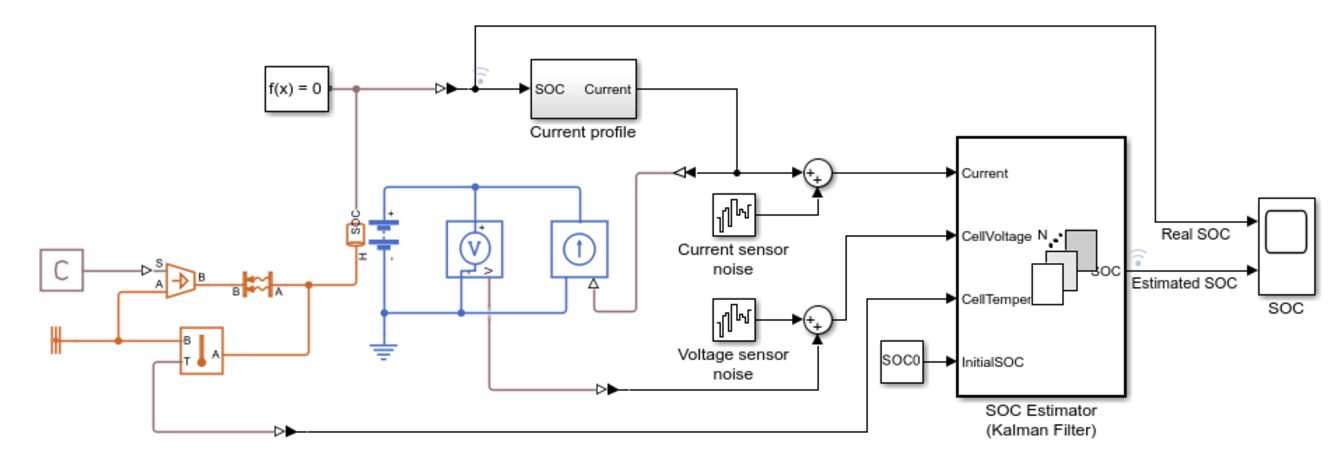
\includegraphics[width=1\textwidth]{imgs/simulink_EKF.png}
\caption{MATLAB Simulink implementation of Extended Kalman Filter for battery state-of-charge estimation, showing the complete simulation framework used for testing and validation.}
\label{fig:simulink_ekf_implementation}
\end{figure}

To enhance the accuracy and realism of the simulations, the standard battery block was replaced with the Batemo INR21700-p45b model, which was accessible through the Formula Student team collaboration at the polytechnic. The Batemo model~\cite{batemo_website_2024} offers a highly accurate, physics-based battery simulation with its own dedicated Simulink block, enabling realistic testing conditions and validation of the proposed approaches. Figure~\ref{fig:batemo_blocks} illustrates the block diagram structure of the Batemo battery model integration.

\begin{figure}[htbp]
\centering
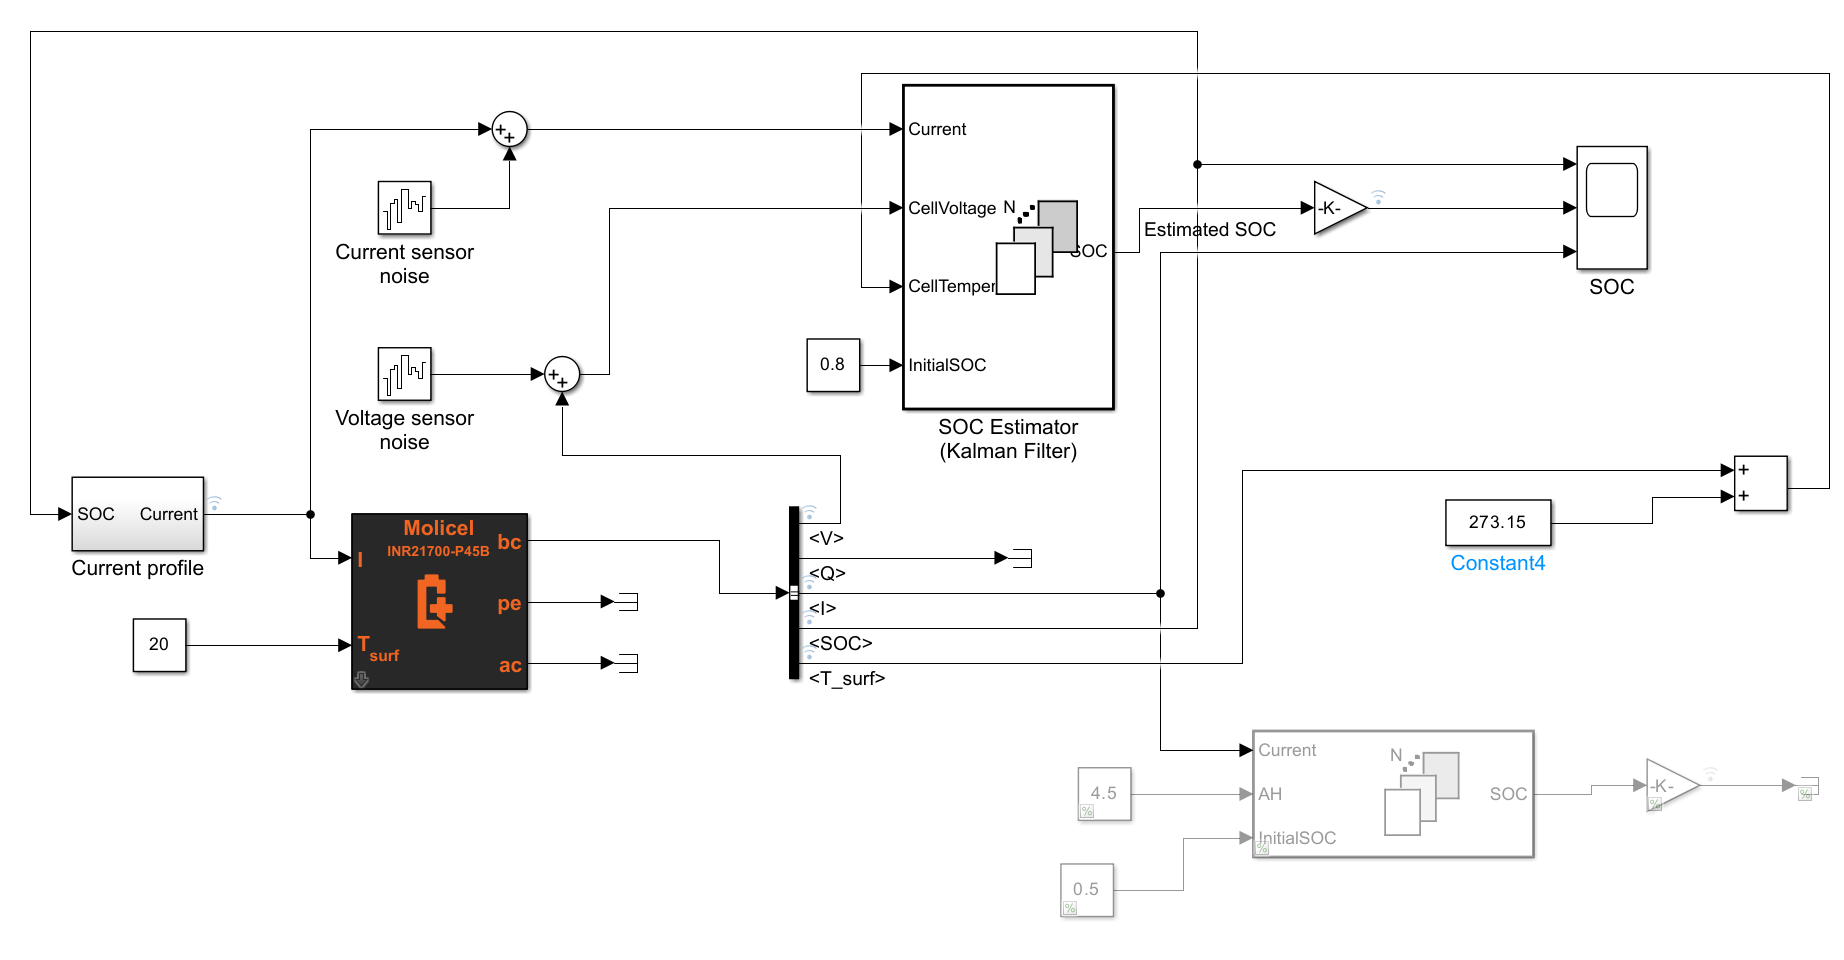
\includegraphics[width=0.8\textwidth]{imgs/batemo_blocks.png}
\caption{Block diagram of the Batemo INR21700-p45b battery model integration, showing the physics-based simulation structure used for enhanced accuracy in battery behavior modeling.}
\label{fig:batemo_blocks}
\end{figure}

First, the EKF was implemented as the primary estimation algorithm for SOC prediction. The EKF approach was chosen for its proven effectiveness in handling the nonlinear behavior of battery systems and its ability to provide uncertainty measurement. Coulomb counting was integrated as a supporting method for SOC estimation, providing a reference baseline for comparison with the Kalman filter results. Figure~\ref{fig:ekf_results} presents the estimation results obtained from the EKF implementation, demonstrating the algorithm's performance in tracking battery SOC.

\begin{figure}[htbp]
\centering
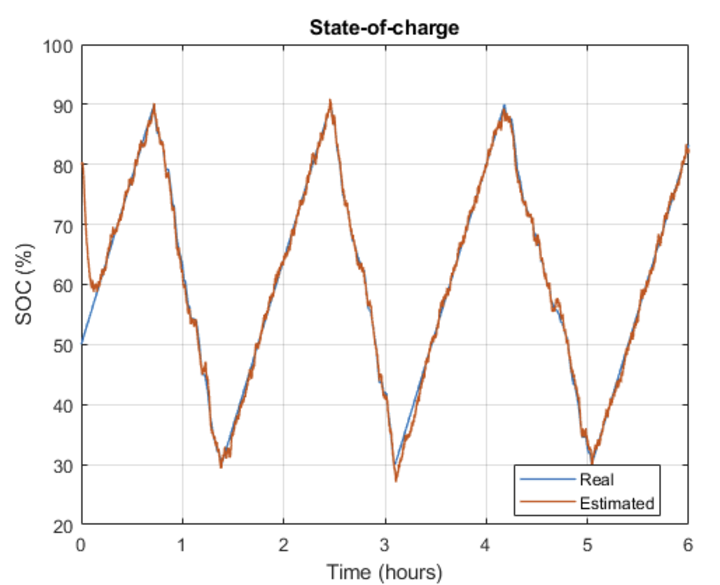
\includegraphics[width=0.9\textwidth]{imgs/EKF_results.png}
\caption{Extended Kalman Filter estimation results showing SOC tracking performance and comparison with reference measurements, illustrating the accuracy and reliability of the implemented algorithm.}
\label{fig:ekf_results}
\end{figure} 

The implementation addressed several critical considerations to ensure accuracy and reliability. \textbf{Current integration accuracy and drift compensation} were prioritized to minimize cumulative errors that could significantly impact SOC estimates over extended periods. \textbf{Temperature effects} were carefully analyzed, as thermal variations can substantially alter the charge-discharge efficiency and affect the accuracy of capacity calculations. \textbf{Aging effects on capacity estimation} were incorporated to account for the gradual degradation of battery capacity over operational lifetime, ensuring that SOC estimates remain accurate as the battery ages. Finally, \textbf{calibration procedures for initial SOC} were established to provide accurate baseline measurements, which are crucial for the cumulative nature of coulomb counting methods.

The Batemo battery model was incorporated to provide physics-based battery behavior simulation. This integration offered complete capabilities for model development and validation. Figure~\ref{fig:batemo_configurations} shows the detailed configuration options available in the Batemo model, while Figure~\ref{fig:batemo_estimation} demonstrates the estimation capabilities achieved through the physics-based simulation approach.

\begin{figure}[htbp]
\centering
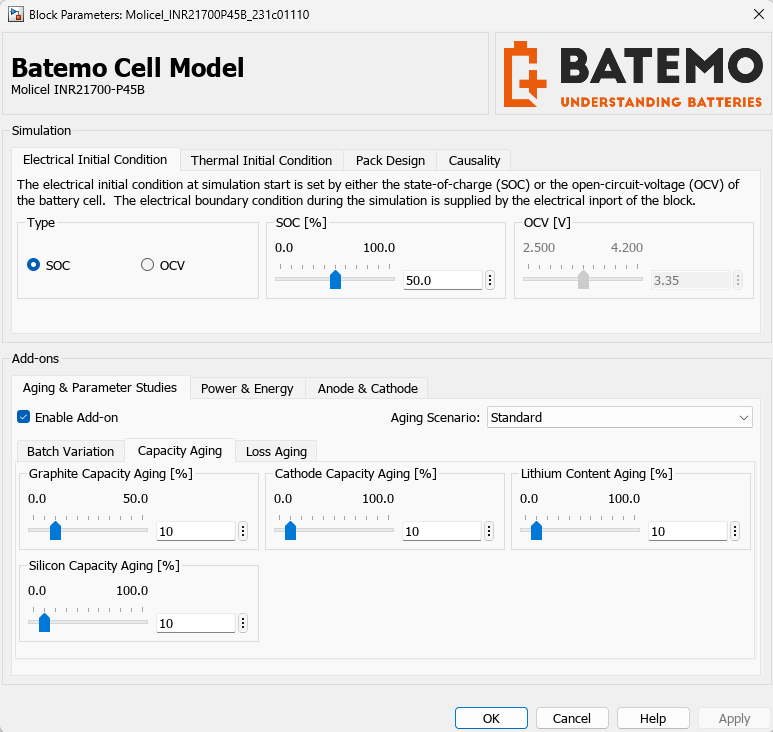
\includegraphics[width=0.8\textwidth]{imgs/batemo_configurations.png}
\caption{Batemo battery model configuration interface, showing the various agging and batterry parameters}
\label{fig:batemo_configurations}
\end{figure}

\begin{figure}[htbp]
\centering
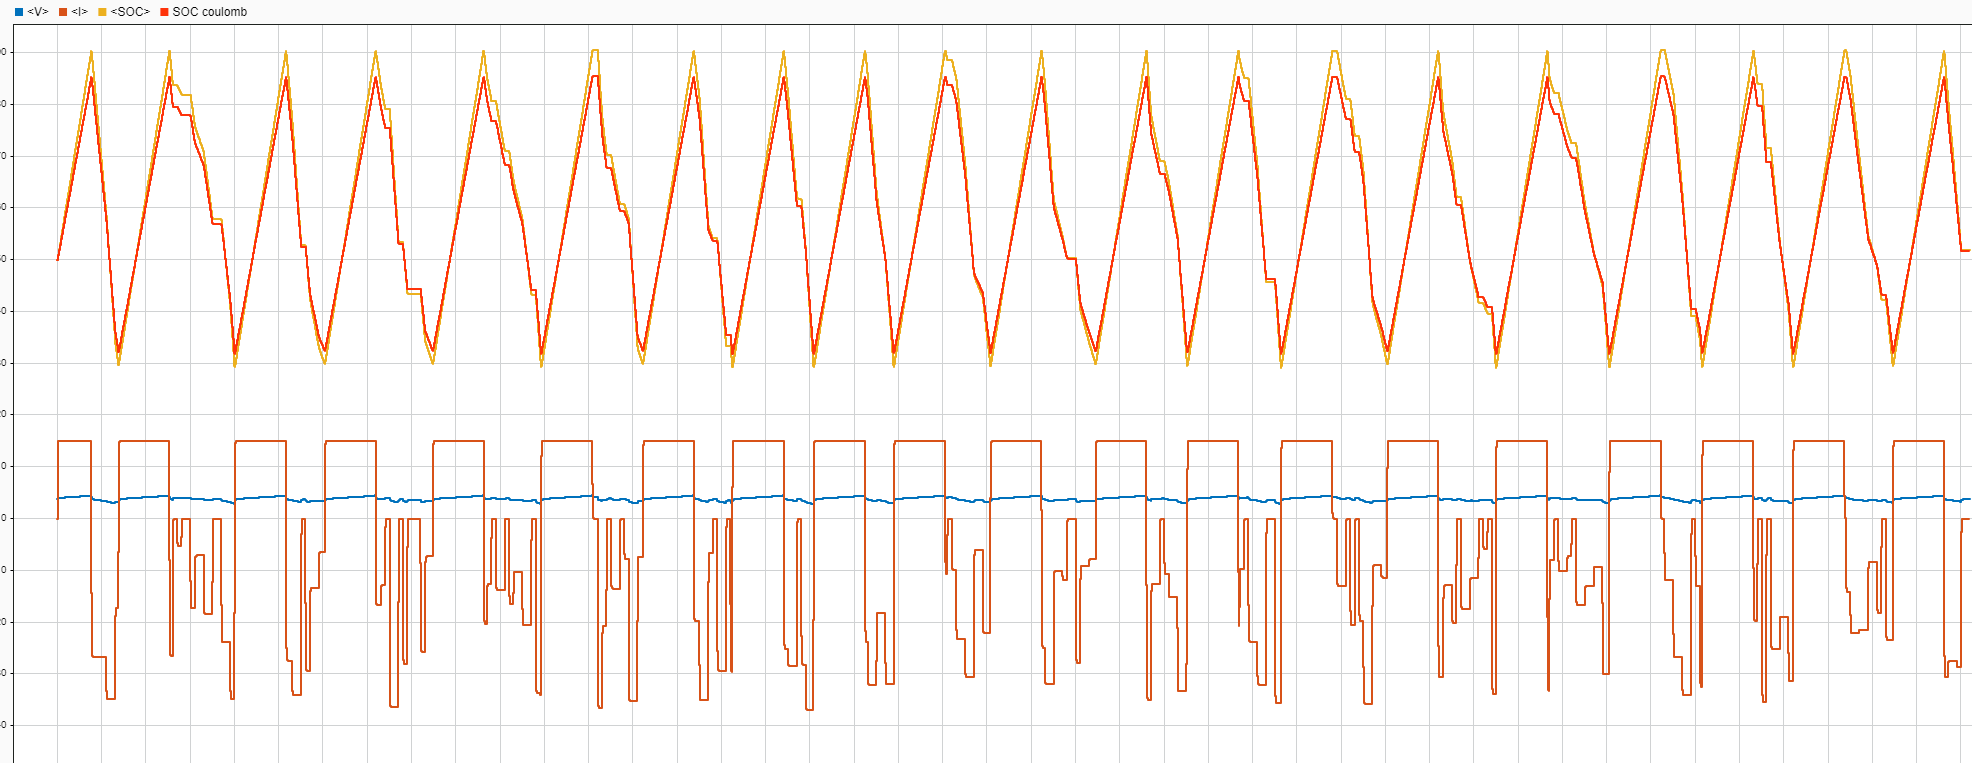
\includegraphics[width=0.9\textwidth]{imgs/batemo_estimation.png}
\caption{Battery state estimation results obtained using the Batemo physics-based model, demonstrating improved accuracy compared to standard battery models. The top graph shows the estimated SOC (orange line) compared with the actual SOC (yellow line).}
\label{fig:batemo_estimation}
\end{figure}

\textbf{Validation of estimation algorithms under controlled conditions} was enabled through the model's ability to simulate battery behaviors, allowing for systematic testing of algorithm performance across various operational scenarios. \textbf{Potential for synthetic data generation} was identified as a valuable capability for training and evaluating neural networks when real world data is limited, though this approach was not pursued in favor of using real data datasets. \textbf{Analysis of model sensitivity to various degradation mechanisms} was made possible by the physics-based nature of the Batemo model, enabling detailed investigation of how different aging phenomena affect battery performance predictions. 

This MATLAB implementation served as a foundation for understanding battery dynamics and provided insights that informed subsequent neural network development phases. The experience gained from working with both simulated and physics-based models highlighted the importance of high-quality data and the potential benefits of combining model-based insights with data-driven approaches.

\section{Neural Network Approaches}
\label{sec:neural_network_evolution}

This work evaluated different NN approaches, each addressing specific limitations identified in others and incorporating lessons learned from the MATLAB modeling phase.

%\subsection{Hybrid (CNN + LSTM) Architecture}
%\label{subsec:cnn_lstm_architecture}
%
%The first neural network implementation combined CNN with LSTM networks to leverage both spatial feature extraction and temporal sequence modeling capabilities\color{Red}Referencia da rede que usou\color{Black}. This CNN+LSTM architecture was structured to use the supporting strengths of both convolutional and recurrent neural networks. The design incorporated multiple specialized layers, each serving a distinct purpose in the feature extraction and temporal modeling pipeline.\color{Red}Ficava bem a referência a uma figura que mostrasse o diagrama de blocos da arquitetura\color{Black} \textbf{CNN layers} were responsible for extracting local patterns and features from battery measurement sequences, identifying spatial relationships and important signal characteristics within the input data. \textbf{LSTM layers} focused on modeling long-term dependencies and temporal relationships, capturing the sequential nature of battery degradation and state evolution over time. Finally, \textbf{Dense layers} provided the final prediction mapping with appropriate activation functions, transforming the processed features into accurate SOC and SOH estimates.
%
%Several significant challenges were encountered during the implementation that highlighted the complexity of applying deep learning to battery health monitoring. These obstacles required careful analysis and ultimately influenced the decision to pursue alternative approaches. \textbf{Gradient vanishing} emerged as a critical issue where long sequences caused training instability, preventing the network from effectively learning long-term dependencies essential for accurate battery state prediction. \textbf{Overfitting} presented another major concern, as the high model complexity led to poor generalization, with the network memorizing training patterns rather than learning transferable features applicable to new battery data. \textbf{Computational efficiency} posed practical limitations, with training time becoming too long for large datasets, making the approach unsuitable for real world applications requiring timely model updates. Additionally, \textbf{Feature engineering} proved challenging, as manual feature selection proved suboptimal, requiring extensive domain expertise and iterative refinement that limited the model's adaptability to different battery types and operating conditions.
%
%\subsection{Hybrid vs. Data-Driven Approach Evaluation}
%\label{subsec:hybrid_vs_datadriven}
%
%A systematic comparison was conducted between hybrid approaches (combining physics-based models with neural networks) and pure data-driven methods.\color{Red}Tem de dizer que modelos experimentou em cada uma das abordagens, indicando referências e apresentando figuras \color{Black}
%
%The hybrid approach integrated multiple supporting techniques to use both physics-based understanding and data-driven learning capabilities. This complete strategy incorporated several key components designed to enhance prediction accuracy and reliability. \textbf{Physics-based model outputs as additional input features} provided domain-specific insights that enriched the neural network's understanding of battery behavior, incorporating basic electrochemical principles into the learning process. \textbf{Kalman filter estimates as regularization terms} helped constrain the neural network training by incorporating well-established state estimation techniques, reducing the likelihood of unrealistic predictions and improving model stability. Furthermore, \textbf{domain knowledge constraints in loss function design} ensured that the learned models respected known physical limitations and relationships, preventing the network from learning patterns that violated basic battery physics principles.
%
%The pure data-driven approach emphasized maximum use of machine learning capabilities while minimizing reliance on explicit domain knowledge. This methodology focused on allowing the neural network to discover patterns and relationships directly from the data. \textbf{End-to-end learning from raw sensor data} enabled the model to process unfiltered battery measurements, potentially capturing subtle patterns that might be lost during manual preprocessing or feature engineering steps. \textbf{Automatic feature extraction and representation learning} allowed the network to identify the most relevant characteristics for battery health prediction without requiring extensive domain expertise or manual feature design. Additionally, \textbf{minimal domain-specific preprocessing requirements} reduced implementation complexity and improved the method's adaptability to different battery types and measurement configurations, making it more suitable for diverse real world applications.
%
%The evaluation revealed that data-driven approaches demonstrated \textbf{better generalization} across different battery chemistries, \textbf{reduced dependency} on accurate physics model parameters, \textbf{better scalability} to large datasets, and \textbf{more strong performance} under varying operating conditions. This analysis motivated the transition to advanced pure data-driven architectures, which require the use of comprehensive and high-quality datasets.

\subsection{Transformer and Mixture of Experts Networks}
\label{subsec:transformer_moe_networks}

During the literature review process, the Transformer network for Remaining Useful Life prediction of lithium-ion batteries~\cite{chen_transformer_2022} was identified as a promising approach that demonstrated superior performance for battery health prediction tasks. This work introduced a Transformer-based neural network specifically designed for battery RUL prediction using the CALCE dataset \cite{CALCE_battery_nodate}.

The paper addressed the challenge of noisy battery capacity data through a two-stage framework. First, a Denoising Auto-Encoder(DAE) was applied to process the raw battery data and reduce noise commonly present during charge-discharge cycles. The denoised data was then fed into a Transformer network to capture temporal information and learn features relevant to battery degradation patterns. The unified framework combined both denoising and prediction tasks, enabling accurate RUL estimation.

The Transformer architecture utilized self-attention mechanisms to model long-range dependencies in battery degradation sequences, effectively capturing relationships between distant time points in the battery operational history. This approach demonstrated superior performance compared to traditional methods on multiple battery datasets, showing improved accuracy in predicting both SOH and EOL estimates. Figure~\ref{fig:transformer_architecture} illustrates the complete Transformer architecture implemented for battery RUL prediction, showing the multi-head attention mechanisms and feed-forward layers that enable effective temporal pattern recognition.

\begin{figure}[htbp]
\centering
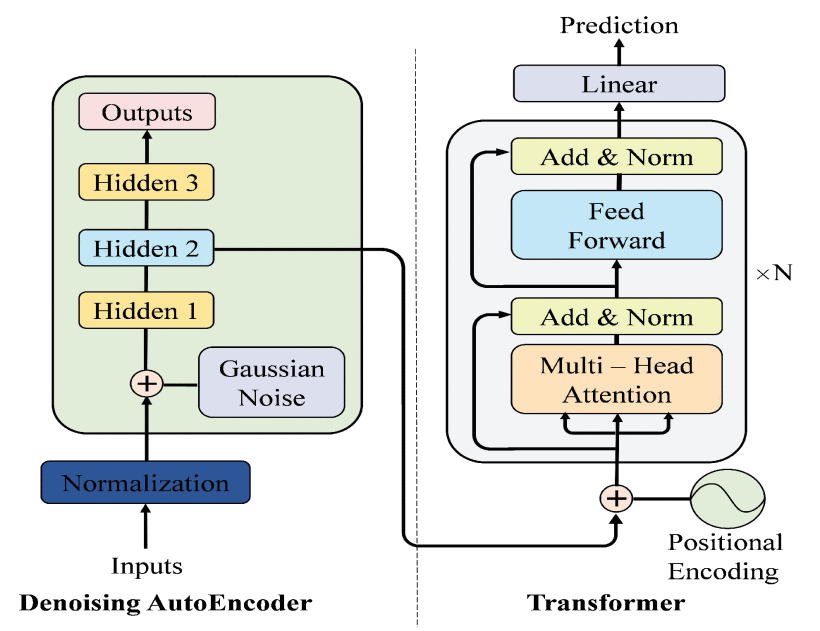
\includegraphics[width=0.9\textwidth]{imgs/transformer_arq.png}
\caption{Transformer architecture for battery RUL prediction, showing the self-attention mechanisms and encoder-decoder structure that enables modeling of long-range dependencies in battery degradation sequences\cite{chen_transformer_2022}.}
\label{fig:transformer_architecture}
\end{figure}

Building on concepts from Transferred Multi-Task Learning \cite{che_battery_2023}, which showed promise for battery state monitoring across different operating conditions, an investigation into Mixture of Experts(MoE) networks was conducted. MoE represents a powerful neural network architecture that combines multiple specialized sub-networks (experts) with a gating mechanism that determines which experts should be activated for each input sample.

The MoE architecture offers several advantages for battery health prediction:

\begin{itemize}
    \item \textbf{Specialized learning}: Different experts can focus on specific battery degradation modes or operating conditions
    \item \textbf{Computational efficiency}: Only a subset of experts are activated for each prediction, reducing computational overhead
    \item \textbf{Feature-specific tuning}: Experts can be optimized for different input features (voltage, current, temperature)
    \item \textbf{Scalable capacity}: Model capacity can be increased by adding experts without proportional computational cost increase
\end{itemize}

To evaluate the effectiveness of MoE networks for battery RUL prediction, the same experimental setup as the Transformer paper was replicated, but with the Transformer architecture replaced by a MoE network. The MoE implementation consisted of three specialized experts and a learned gating network that dynamically weighted expert contributions based on input characteristics. Figure~\ref{fig:moe_architecture} presents the detailed architecture of the implemented MoE network, highlighting the gating mechanism and expert specialization.

\begin{figure}[htbp]
\centering
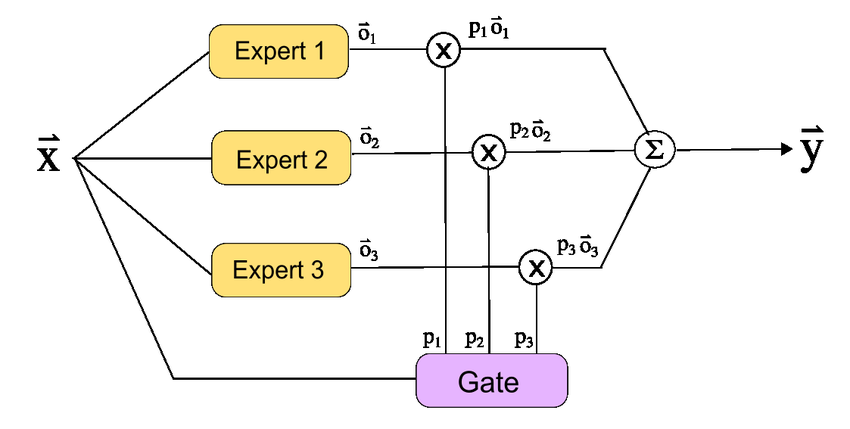
\includegraphics[width=0.9\textwidth]{imgs/Moe_arq.png}
\caption{MoE architecture for battery health prediction, showing the gating network and specialized experts that enable efficient learning of different battery degradation patterns and operating conditions~\cite{moe_arq}.}
\label{fig:moe_architecture}
\end{figure}


\begin{figure}[htbp]
    \centering
    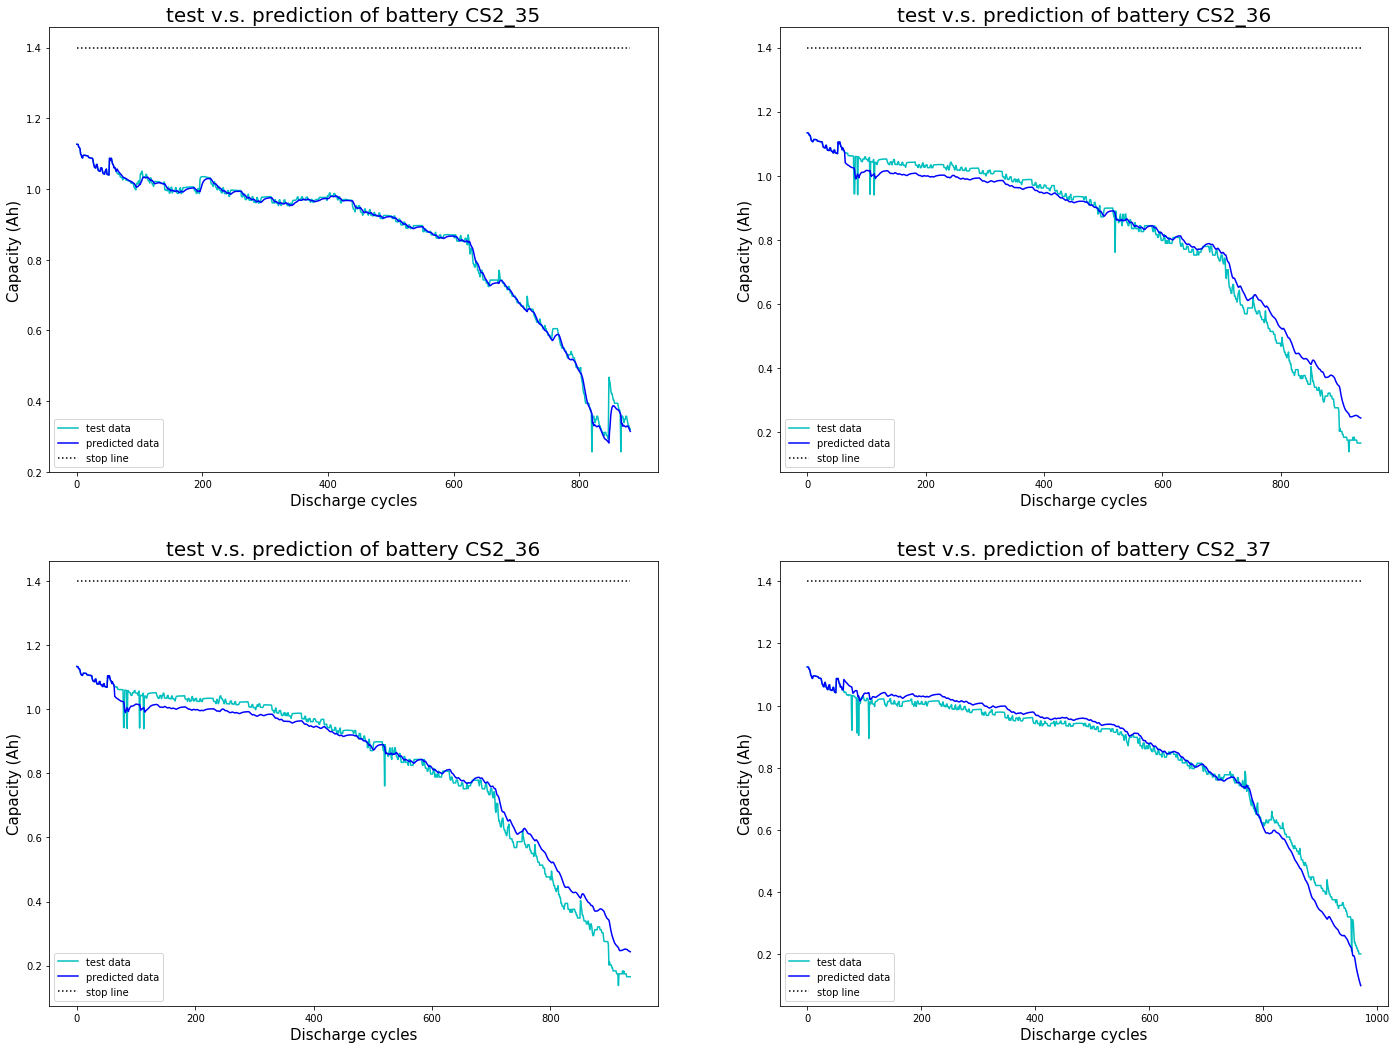
\includegraphics[width=0.9\textwidth]{imgs/transf_graph_results.png}
    \caption{Transformer network performance results for battery RUL prediction on CALCE dataset, showing prediction accuracy and convergence behavior during training and validation phases.}
    \label{fig:transformer_results}
\end{figure}


\begin{figure}[htbp]
    \centering
    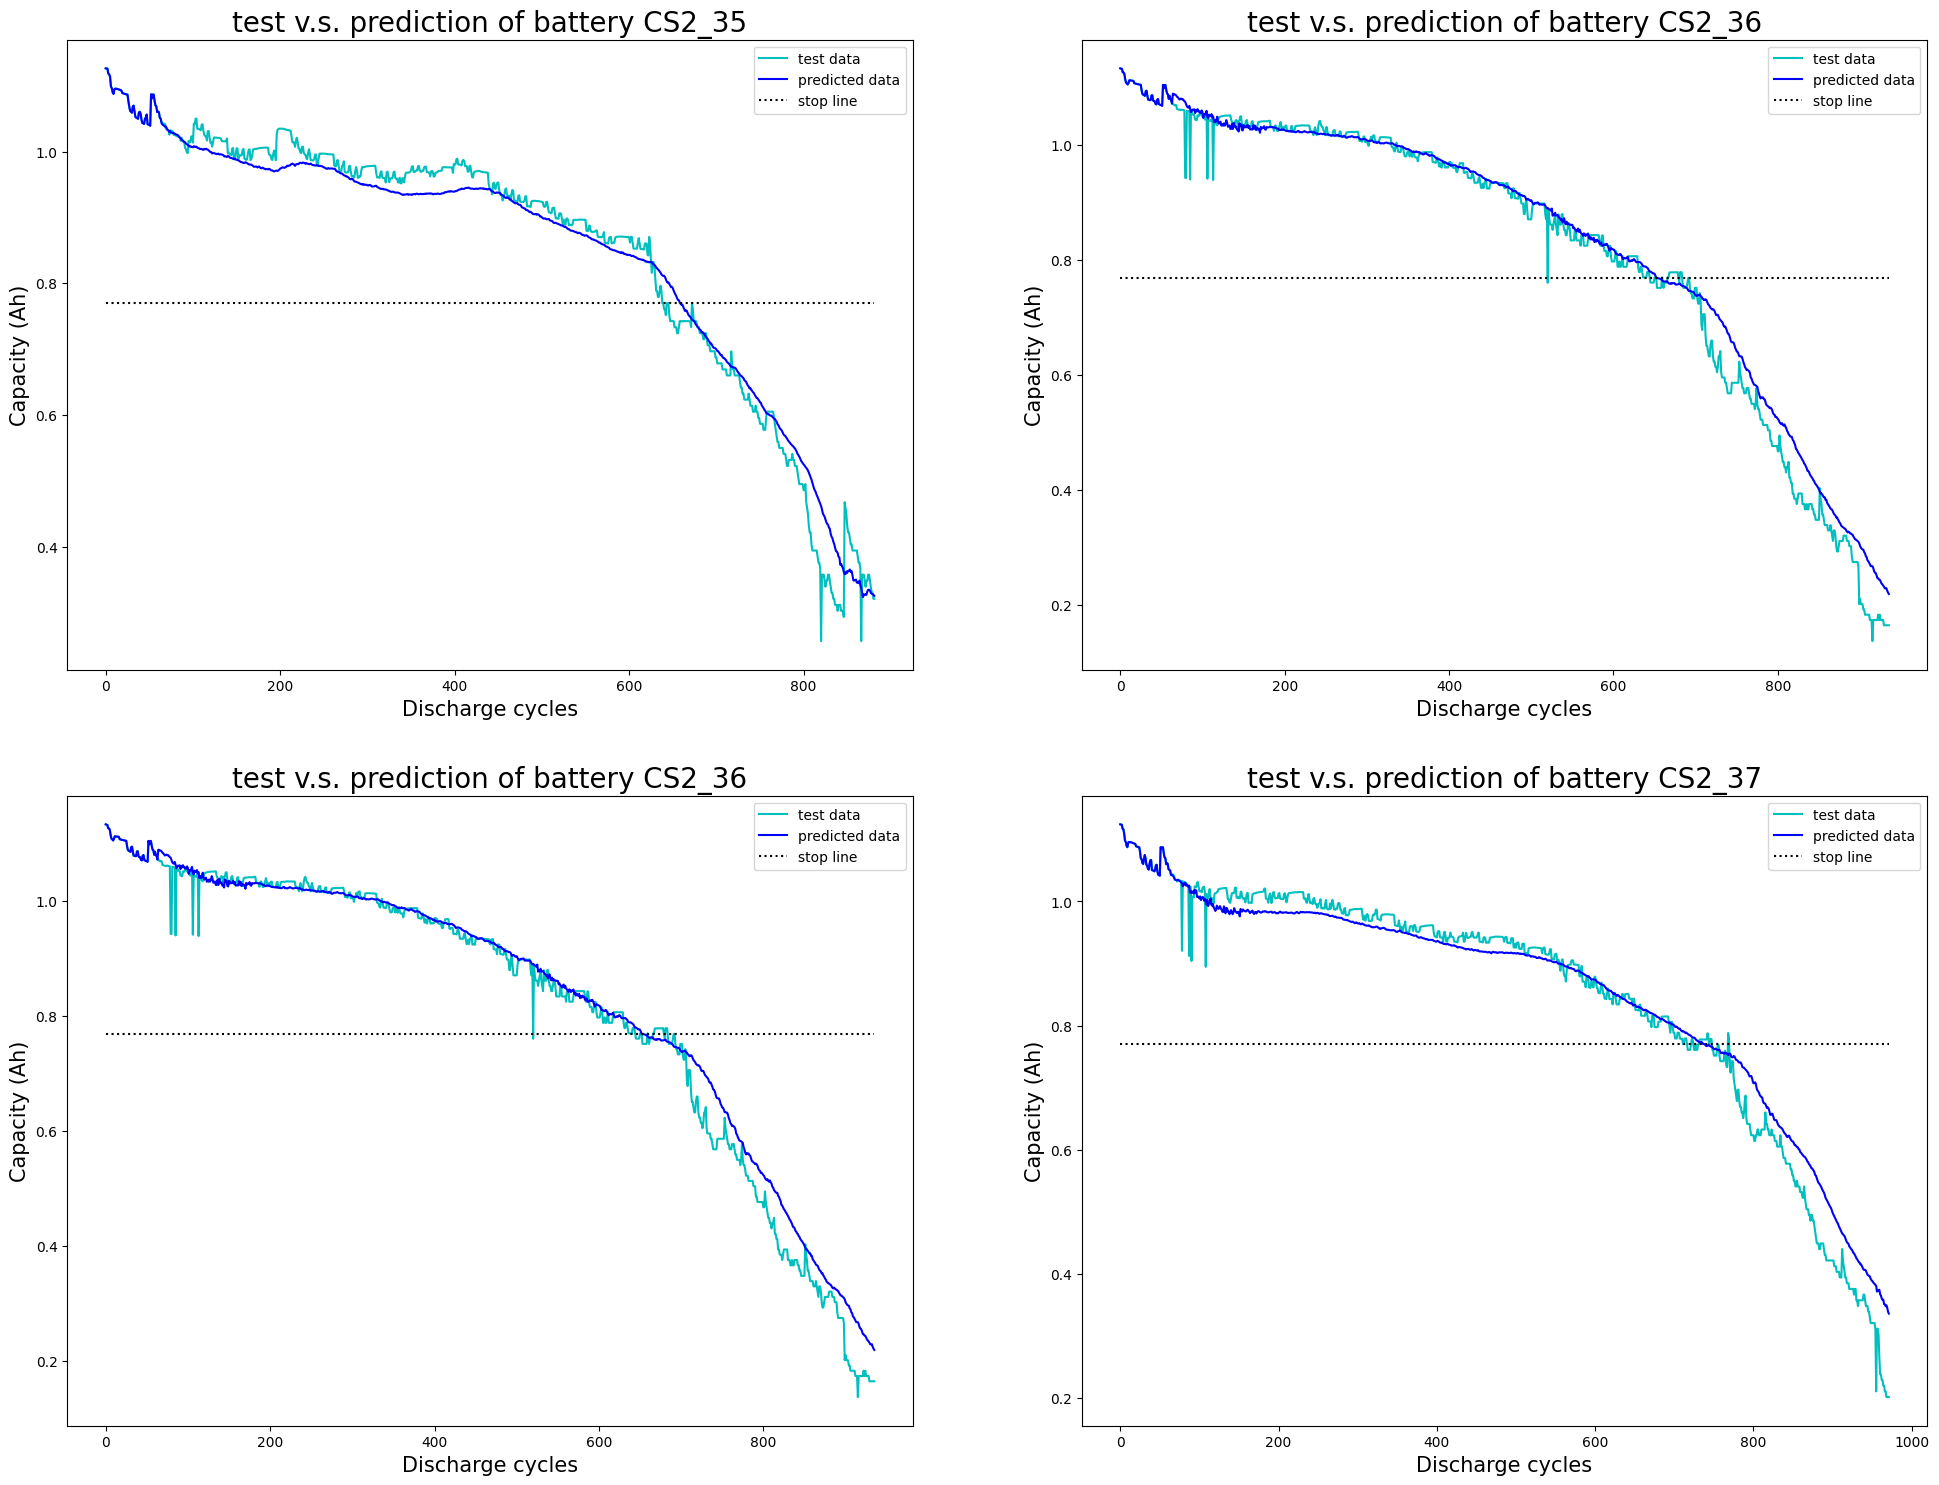
\includegraphics[width=0.9\textwidth]{imgs/moe_graph_results.png}
    \caption{MoE network performance results for battery RUL prediction, demonstrating competitive accuracy with reduced computational complexity compared to the Transformer approach.}
    \label{fig:moe_results}
\end{figure}

\begin{table}[htbp]
    \centering
    \caption{Quantitative comparison of Transformer vs. MoE network performance for battery RUL prediction}
    \label{tab:transformer_moe_results}
    \begin{tabular}{lc}
        \hline
        \textbf{Model} & \textbf{RMSE} \\
        \hline
        Transformer & 0.0297 \\
        FCN MoE & 0.0335 \\
        \hline
    \end{tabular}
\end{table}

The experimental results demonstrated that a simple MoE network with just three experts could achieve performance levels comparable to the much more complex Transformer-based architecture. Figure~\ref{fig:transformer_results} shows the training and validation performance of the Transformer network, while Figure~\ref{fig:moe_results} presents the corresponding results for the MoE implementation. Table~\ref{tab:transformer_moe_results} provides a quantitative comparison of the two approaches, showing that while the Transformer model achieved a slightly better RMSE of 0.0297 compared to the FCN MoE network's 0.0335, the MoE network provided competitive results with significantly reduced model complexity and computational requirements.


This experiment demonstrated the potential of MoE networks as an efficient alternative to complex Transformer architectures for battery health prediction tasks, offering a good balance between prediction accuracy and computational efficiency.

\section{Dataset Collection and Preprocessing}
\label{sec:dataset_preprocessing}

The CALCE battery dataset was selected as the primary dataset for this work due to its comprehensive feature set and established use in the battery research community.

\subsection{Dataset Characteristics and Features}
\label{subsec:dataset_characteristics}

The CALCE dataset contains multiple battery cells subjected to complete discharge-charge cycling until EOL under various current profiles. For this study, the CS2 battery cell was selected, which was cycled at a constant current rate of 0.5C. This particular cell provides 886 CSV files containing battery cycle data. The original dataset is organized in batches of 50 cycles each, with the first cycle of each batch removed to eliminate initialization artifacts. A custom made Python script was developed to separate all cycles into individual files, sequentially numbered from 1.csv to 886.csv.

\begin{figure}[htbp]
\centering
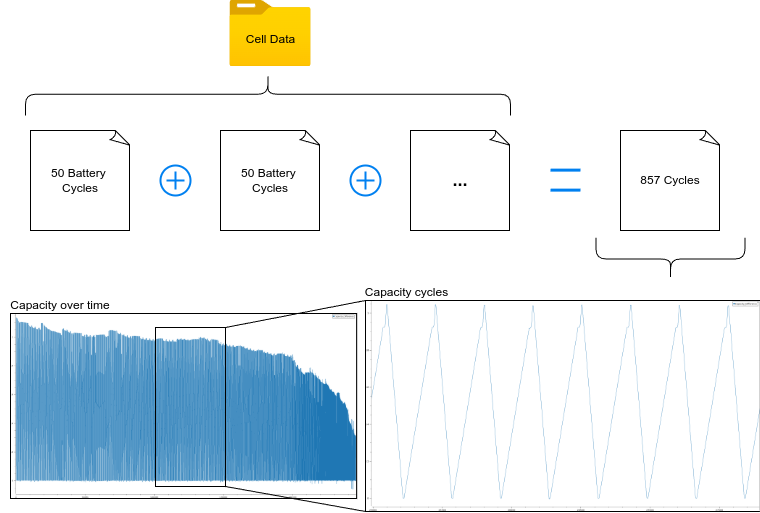
\includegraphics[width=1.0\textwidth]{imgs/cycles_files.png}
\caption{Dataset structure showing the systematic organization of battery cycle data from batches to individual files.}
\label{fig:dataset_structure}
\end{figure}

The original data contains multiple features including capacity, energy, current, voltage, and resistance measurements. Through preprocessing, the dataset is streamlined to focus on essential variables: Capacity\_Difference, Cumulative\_Cycle\_Index, Current(A), Date\_Time, RUL, SOC, SOH, and Voltage(V).

\subsubsection{SOC Calculation}
\label{subsubsec:soc_calculation}

SOC is calculated using a cycle-relative approach for each charge-discharge cycle:

\begin{enumerate}
    \item \textbf{Cycle-based maximum capacity determination}: For each cycle, the maximum discharge capacity is identified using:
    \begin{equation}
        C_{max,cycle} = \max(\text{Reset\_Discharge\_Capacity}_{cycle})
    \end{equation}
    
    \item \textbf{Instantaneous SOC calculation}: The SOC at any given time point is calculated as:
    \begin{equation}
        SOC = \frac{\text{Reset\_Discharge\_Capacity}}{\text{Cycle\_Max\_Discharge}} \times 100\%
    \end{equation}
    
    SOC values are clipped to ensure they remain within the physically meaningful range of 0-100\%.
\end{enumerate}

This approach ensures that SOC represents the true charge state within each cycle, providing accurate representation of the battery's operational state regardless of capacity degradation over time.

\subsubsection{SOH Calculation}
\label{subsubsec:soh_calculation}

The SOH calculation provides a measure of the battery's current capacity relative to its initial capacity, serving as a key indicator of degradation progression. The calculation process involves:

\begin{enumerate}
    \item \textbf{Cycle maximum capacity extraction}: For each cycle, the maximum discharge capacity is determined:
    \begin{equation}
        C_{max,cycle} = \max(\text{Reset\_Discharge\_Capacity}_{cycle})
    \end{equation}
    
    \item \textbf{Reference capacity establishment}: The overall maximum capacity is identified from all cycles, typically representing the battery's initial capacity:
    \begin{equation}
        C_{reference} = \max(\text{all cycle maximum capacities})
    \end{equation}
    
    \item \textbf{SOH percentage calculation}: The SOH is calculated as:
    \begin{equation}
        SOH = \frac{C_{max,cycle}}{C_{reference}} \times 100\%
    \end{equation}
\end{enumerate}

This methodology ensures that SOH accurately reflects the battery's capacity retention throughout its operational lifetime, with 100\% representing the initial capacity and declining values indicating progressive degradation.

\subsubsection{RUL Calculation}
\label{subsubsec:rul_calculation}

The RUL calculation provides a predictive metric indicating how much operational life remains before the battery reaches end-of-life conditions. The implementation follows industry-standard practices:

\begin{enumerate}
    \item \textbf{End-of-life threshold definition}: The end-of-life condition is defined as 80\% of initial capacity, following typical industry standards:
    \begin{equation}
        \text{EOL\_threshold} = 80\%
    \end{equation}
    
    \item \textbf{RUL percentage calculation}: The RUL is calculated as a percentage of RUL:
    \begin{equation}
        RUL = \frac{SOH - \text{EOL\_threshold}}{100\% - \text{EOL\_threshold}} \times 100\%
    \end{equation}
    
    RUL values are clipped to ensure they remain within the 0-100\% range, with 0\% indicating end-of-life conditions.
\end{enumerate}

This calculation approach provides a normalized measure of remaining battery life, where 100\% represents a new battery and 0\% indicates that the battery has reached end-of-life conditions. The linear relationship between SOH and RUL enables straightforward interpretation and facilitates machine learning model training.

\subsubsection{Capacity Reset and Tracking}
\label{subsubsec:capacity_tracking}

The accurate calculation of SOC, SOH, and RUL depends on proper capacity tracking throughout battery testing. The implementation includes capacity reset mechanisms:

\begin{enumerate}
    \item \textbf{Step-based capacity reset}: Capacities are reset when the step index reaches 9, indicating the start of a new charge-discharge cycle:
    \begin{equation}
        \text{Reset\_Charge\_Capacity} = 0, \quad \text{Reset\_Discharge\_Capacity} = 0
    \end{equation}
    
    \item \textbf{Incremental capacity tracking}: Capacities are tracked by calculating differences between consecutive measurements:
    \begin{align}
        \Delta C_{charge} &= C_{charge}(t) - C_{charge}(t-1) \\
        \Delta C_{discharge} &= C_{discharge}(t) - C_{discharge}(t-1)
    \end{align}
    
    \item \textbf{Capacity difference calculation}: The net capacity difference is computed to track charge-discharge imbalances:
    \begin{equation}
        \text{Capacity\_Difference} = \text{Reset\_Charge\_Capacity} - \text{Reset\_Discharge\_Capacity}
    \end{equation}
\end{enumerate}

This approach ensures that all capacity-based calculations maintain accuracy throughout the battery's operational history, providing foundation data for SOC, SOH, and RUL.
\subsection{Cycle Selection System}
\label{subsec:cycle_selection_system}

A custom made Python script organizes the 886 CSV files using a group-based selection algorithm. Files are divided into groups of 10, with a 7:2:1 ratio applied within each group for training, validation, and test sets. This yields approximately 70\% training, 20\% validation, and 10\% test data.

\subsubsection{Data Shuffling}

The cycle data are shuffled to prevent the network from memorizing data order and to avoid overfitting. Randomization is implemented with seed-based reproducibility.

\subsection{Data Preprocessing Pipeline}
\label{subsec:preprocessing_pipeline}

Several preprocessing steps ensure data quality: initial cycle removal, incomplete cycle filtering, outlier detection, and data validation. Battery-level partitioning prevents data leakage between training, validation, and test sets.

\subsection{Input Data Structure}
\label{subsec:input_data_structure}

Individual battery cycles are fed to the network in shuffled order. TimesNet automatically discovers periodic patterns and temporal dependencies within this shuffled data using FFT-based period detection and 2D transformation capabilities.

\subsection{Configuration Management and Reproducibility}
\label{subsec:config_management}

The preprocessing pipeline outputs multiple JSON files containing organized file paths for different experimental scenarios. These JSON files include basic selection outputs, distributed subsets, and configurations with specific preprocessing steps applied.
\subsection{Calculated Values Analysis}
\label{subsec:calculated_values_analysis}

Figure~\ref{fig:calculated_values} presents the calculated SOC, SOH, and RUL values across the complete battery dataset, demonstrating the characteristic patterns of battery degradation over operational cycles.

\begin{figure}[htbp]
\centering
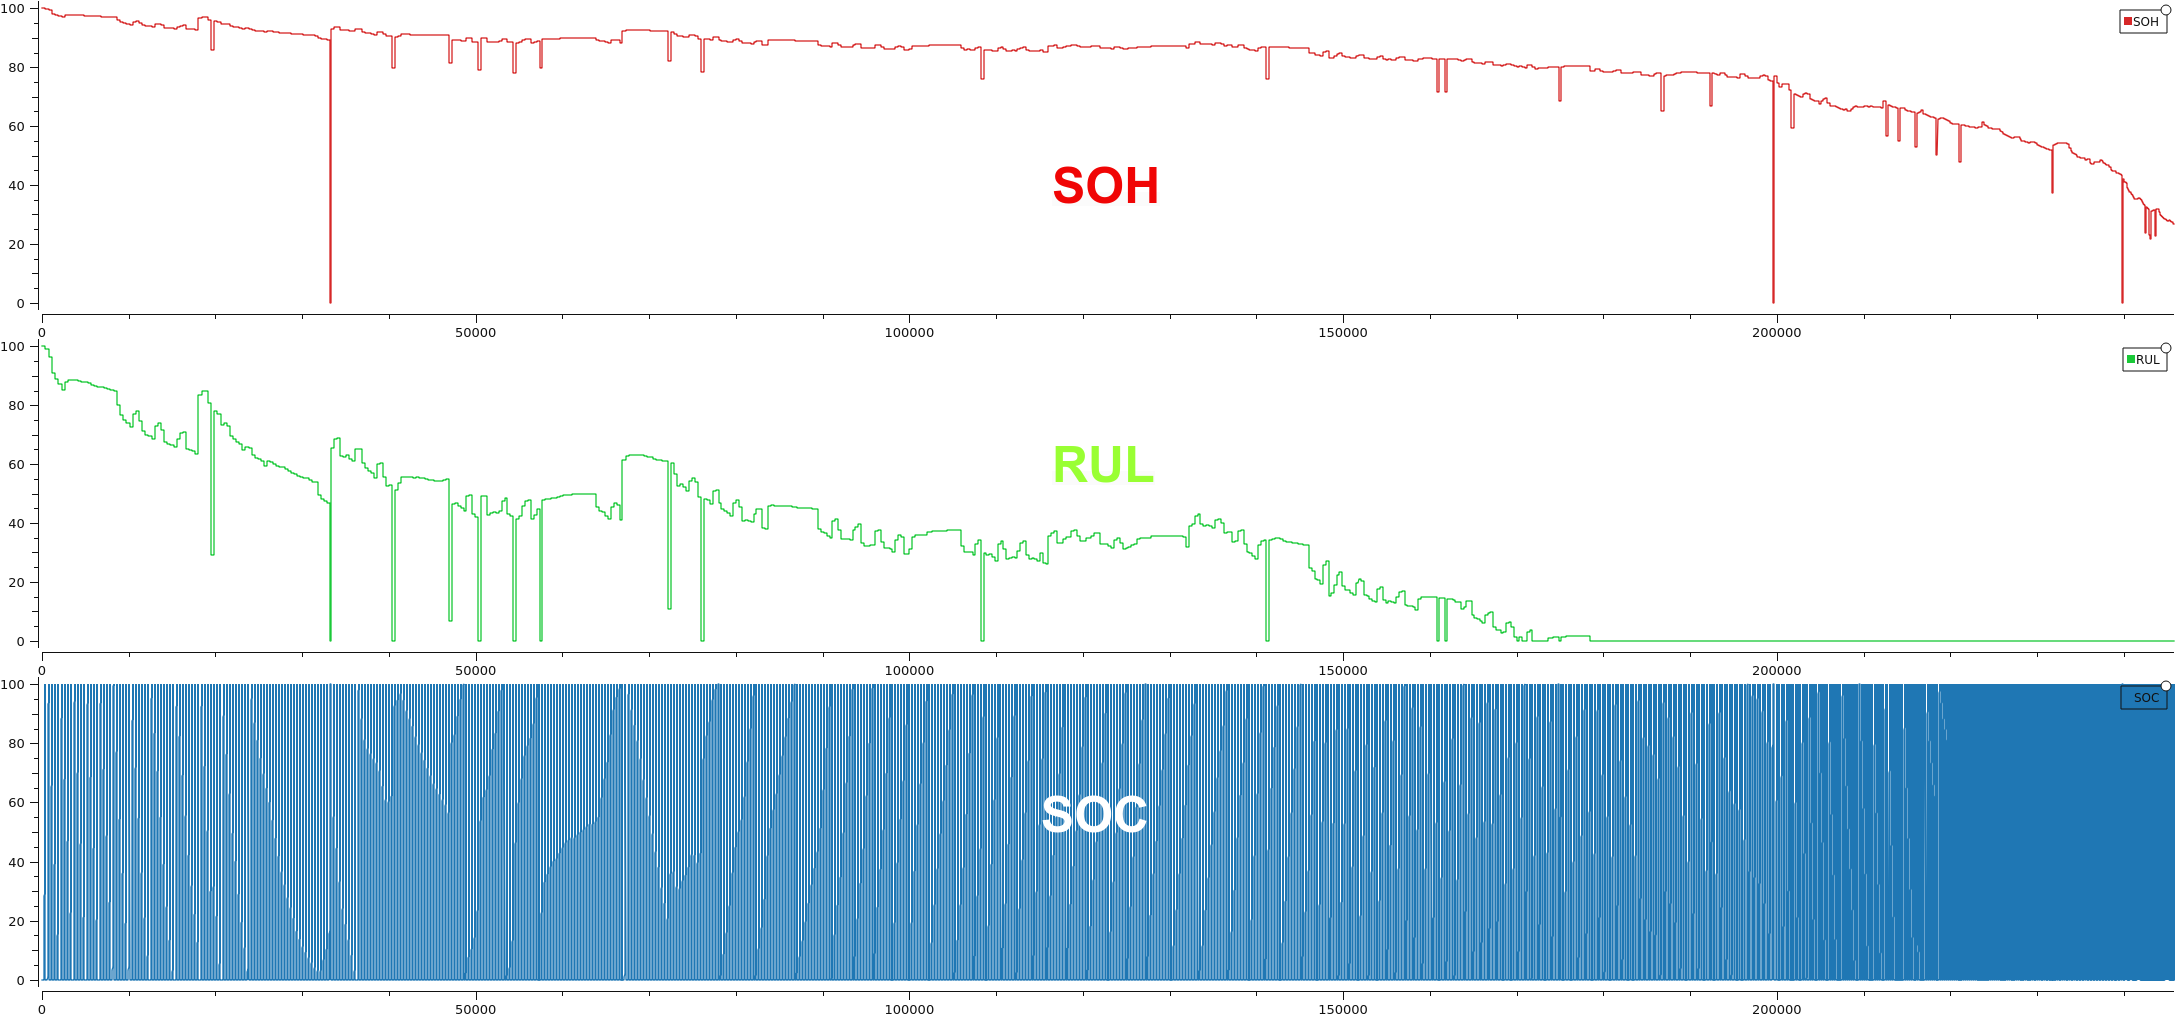
\includegraphics[width=1.0\textwidth]{imgs/soc_soh_rul.png}
\caption{Calculated SOC, SOH, and RUL values across battery operational cycles, showing the characteristic patterns of battery degradation and state evolution.}
\label{fig:calculated_values}
\end{figure}

The results demonstrate three distinct behavioral patterns that are fundamental to battery health monitoring:

\textbf{SOH Degradation}: The SOH values show a clear declining trend as battery cycles progress, starting at 100\% and gradually decreasing to approximately 40\% by the end of the dataset. This degradation pattern reflects the natural capacity fade that occurs in lithium-ion batteries due to various aging mechanisms. The occasional sharp drops in SOH correspond to specific degradation events or measurement artifacts during battery testing.

\textbf{SOC Cycling}: The SOC values exhibit consistent oscillating behavior between 0\% and 100\%, representing the regular charge-discharge cycles throughout battery operation. This cyclic pattern confirms that the SOC calculation correctly captures the charge state variations within each operational cycle, independent of the overall capacity degradation.

\textbf{RUL Decline}: The RUL values demonstrate a progressive decrease as battery cycles advance, starting at 100\% and declining toward 0\% as the battery approaches end-of-life conditions. The RUL calculation effectively translates the SOH degradation into a predictive metric, providing valuable information about the battery's remaining operational capacity.

These patterns validate the accuracy of the implemented calculation methods and provide the foundation for training machine learning models that can predict battery health evolution and RUL based on operational data.

\section{Selected Deep Learning Approach}
\label{sec:timesnet_model}

The evaluation of Transformer and MoE approaches, as described in Section~\ref{subsec:transformer_moe_networks}, provided valuable insights into the strengths and limitations of current state-of-the-art architectures for battery health prediction. While both approaches demonstrated promising results, several critical limitations were identified:

\begin{itemize}
    \item \textbf{Computational complexity}: The Transformer architecture, despite achieving good accuracy (RMSE of 0.0297), required significant computational resources and complex attention mechanisms
    \item \textbf{Limited multi-scale analysis}: Both Transformer and MoE networks struggled to simultaneously capture short-term fluctuations and long-term degradation trends at multiple time scales
    \item \textbf{Period detection limitations}: Manual feature engineering was still required to identify relevant temporal patterns in battery data
    \item \textbf{Generalization constraints}: Performance degradation when applied to battery chemistries or operating conditions not represented in the training data
\end{itemize}

Based on these findings and the need for a more versatile and efficient approach, the following requirements for an improved architecture were identified:

\begin{itemize}
    \item \textbf{Multi-periodicity detection}: Ability to automatically identify and exploit multiple periodic patterns in battery data without manual feature engineering
    \item \textbf{Long-range dependency modeling}: Effective capture of dependencies across extended time horizons while maintaining computational efficiency
    \item \textbf{Parameter efficiency}: Reduced model complexity while maintaining or improving performance compared to Transformer architectures
    \item \textbf{Multi-scale temporal analysis}: Capability to analyze patterns at different time scales simultaneously, from charge-discharge cycles to long-term degradation trends
    \item \textbf{Versatility}: Capability to handle various time series analysis tasks beyond just forecasting
\end{itemize}

These requirements led to the selection and implementation of TimesNet, a cutting-edge architecture specifically designed for general time-series analysis. TimesNet is a modern neural network designed specifically for analyzing time series data~\cite{wu_timesnet_2023}. This model tackles the basic challenge of understanding how data changes over time by converting the complex problem from analyzing 1D time series into analyzing 2D patterns, as illustrated in Figure~\ref{fig:timesnet_2d_transformation}. The key innovation of TimesNet is its ability to discover repeating patterns (periodicity) in time series data and break down complex time changes into smaller, more manageable pieces.


TimesNet starts by analyzing the time series in the frequency domain using FFT to discover multiple periods. real world time series usually present multi-periodicity, such as daily and yearly variations for weather observations, or weekly and quarterly variations for electricity consumption. The period discovery process works by analyzing the frequency spectrum of the input data. The algorithm calculates the amplitude of different frequencies and identifies the strongest periodic patterns by selecting the top-k frequencies with the highest amplitudes. These dominant frequencies correspond to the most important periodic behaviors in the data, such as charge-discharge cycles in battery operations or longer-term capacity fade patterns.


The architecture works by converting 1D time series into a set of 2D grids based on multiple identified periods. This transformation organizes patterns within each period into columns and patterns across different periods into rows of the 2D grids, making time patterns easier to analyze using 2D image processing techniques. Based on the selected frequencies and corresponding period lengths, the 1D time series is reshaped into multiple 2D tensors. This process takes the original time series data and reorganizes it into a grid-like format where each period becomes a row and the progression through different periods becomes columns.

The reshaping process essentially converts temporal patterns into spatial patterns that can be analyzed using 2D image processing techniques. Each identified period creates a separate 2D representation of the data, allowing the model to examine patterns at different time scales simultaneously.
Figure~\ref{fig:timesnet_2d_transformation} illustrates this transformation process, showing how discovering periodicity enables the conversion of original 1D time series into structured 2D tensors that can be processed by 2D kernels conveniently. 

\subsection{TimesBlock Architecture}

The core component, TimesBlock, can automatically discover multiple periods and extract complex time patterns using efficient inception blocks. Each TimesBlock works in a way that preserves the original signal while adding new information, and consists of two main parts:

\begin{enumerate}
\item \textbf{Capturing time patterns in 2D}: After converting the 1D time series into multiple 2D grids, each grid is processed by an efficient inception block that uses different sized filters. This design allows the model to examine patterns at multiple scales - both within individual periods (columns) and across different periods (rows) at the same time.

\item \textbf{Adaptive aggregation}: The k different processed features are combined based on their corresponding amplitudes of the estimated periods. The model uses a weighted combination where stronger periodic patterns (higher amplitudes) have more influence on the final result. This adaptive weighting ensures that the most important temporal patterns dominate the model's predictions.
\end{enumerate}

The shared inception block design makes the model size stay the same regardless of how many periods k are selected, improving efficiency.

\begin{figure}[htbp]
    \centering
    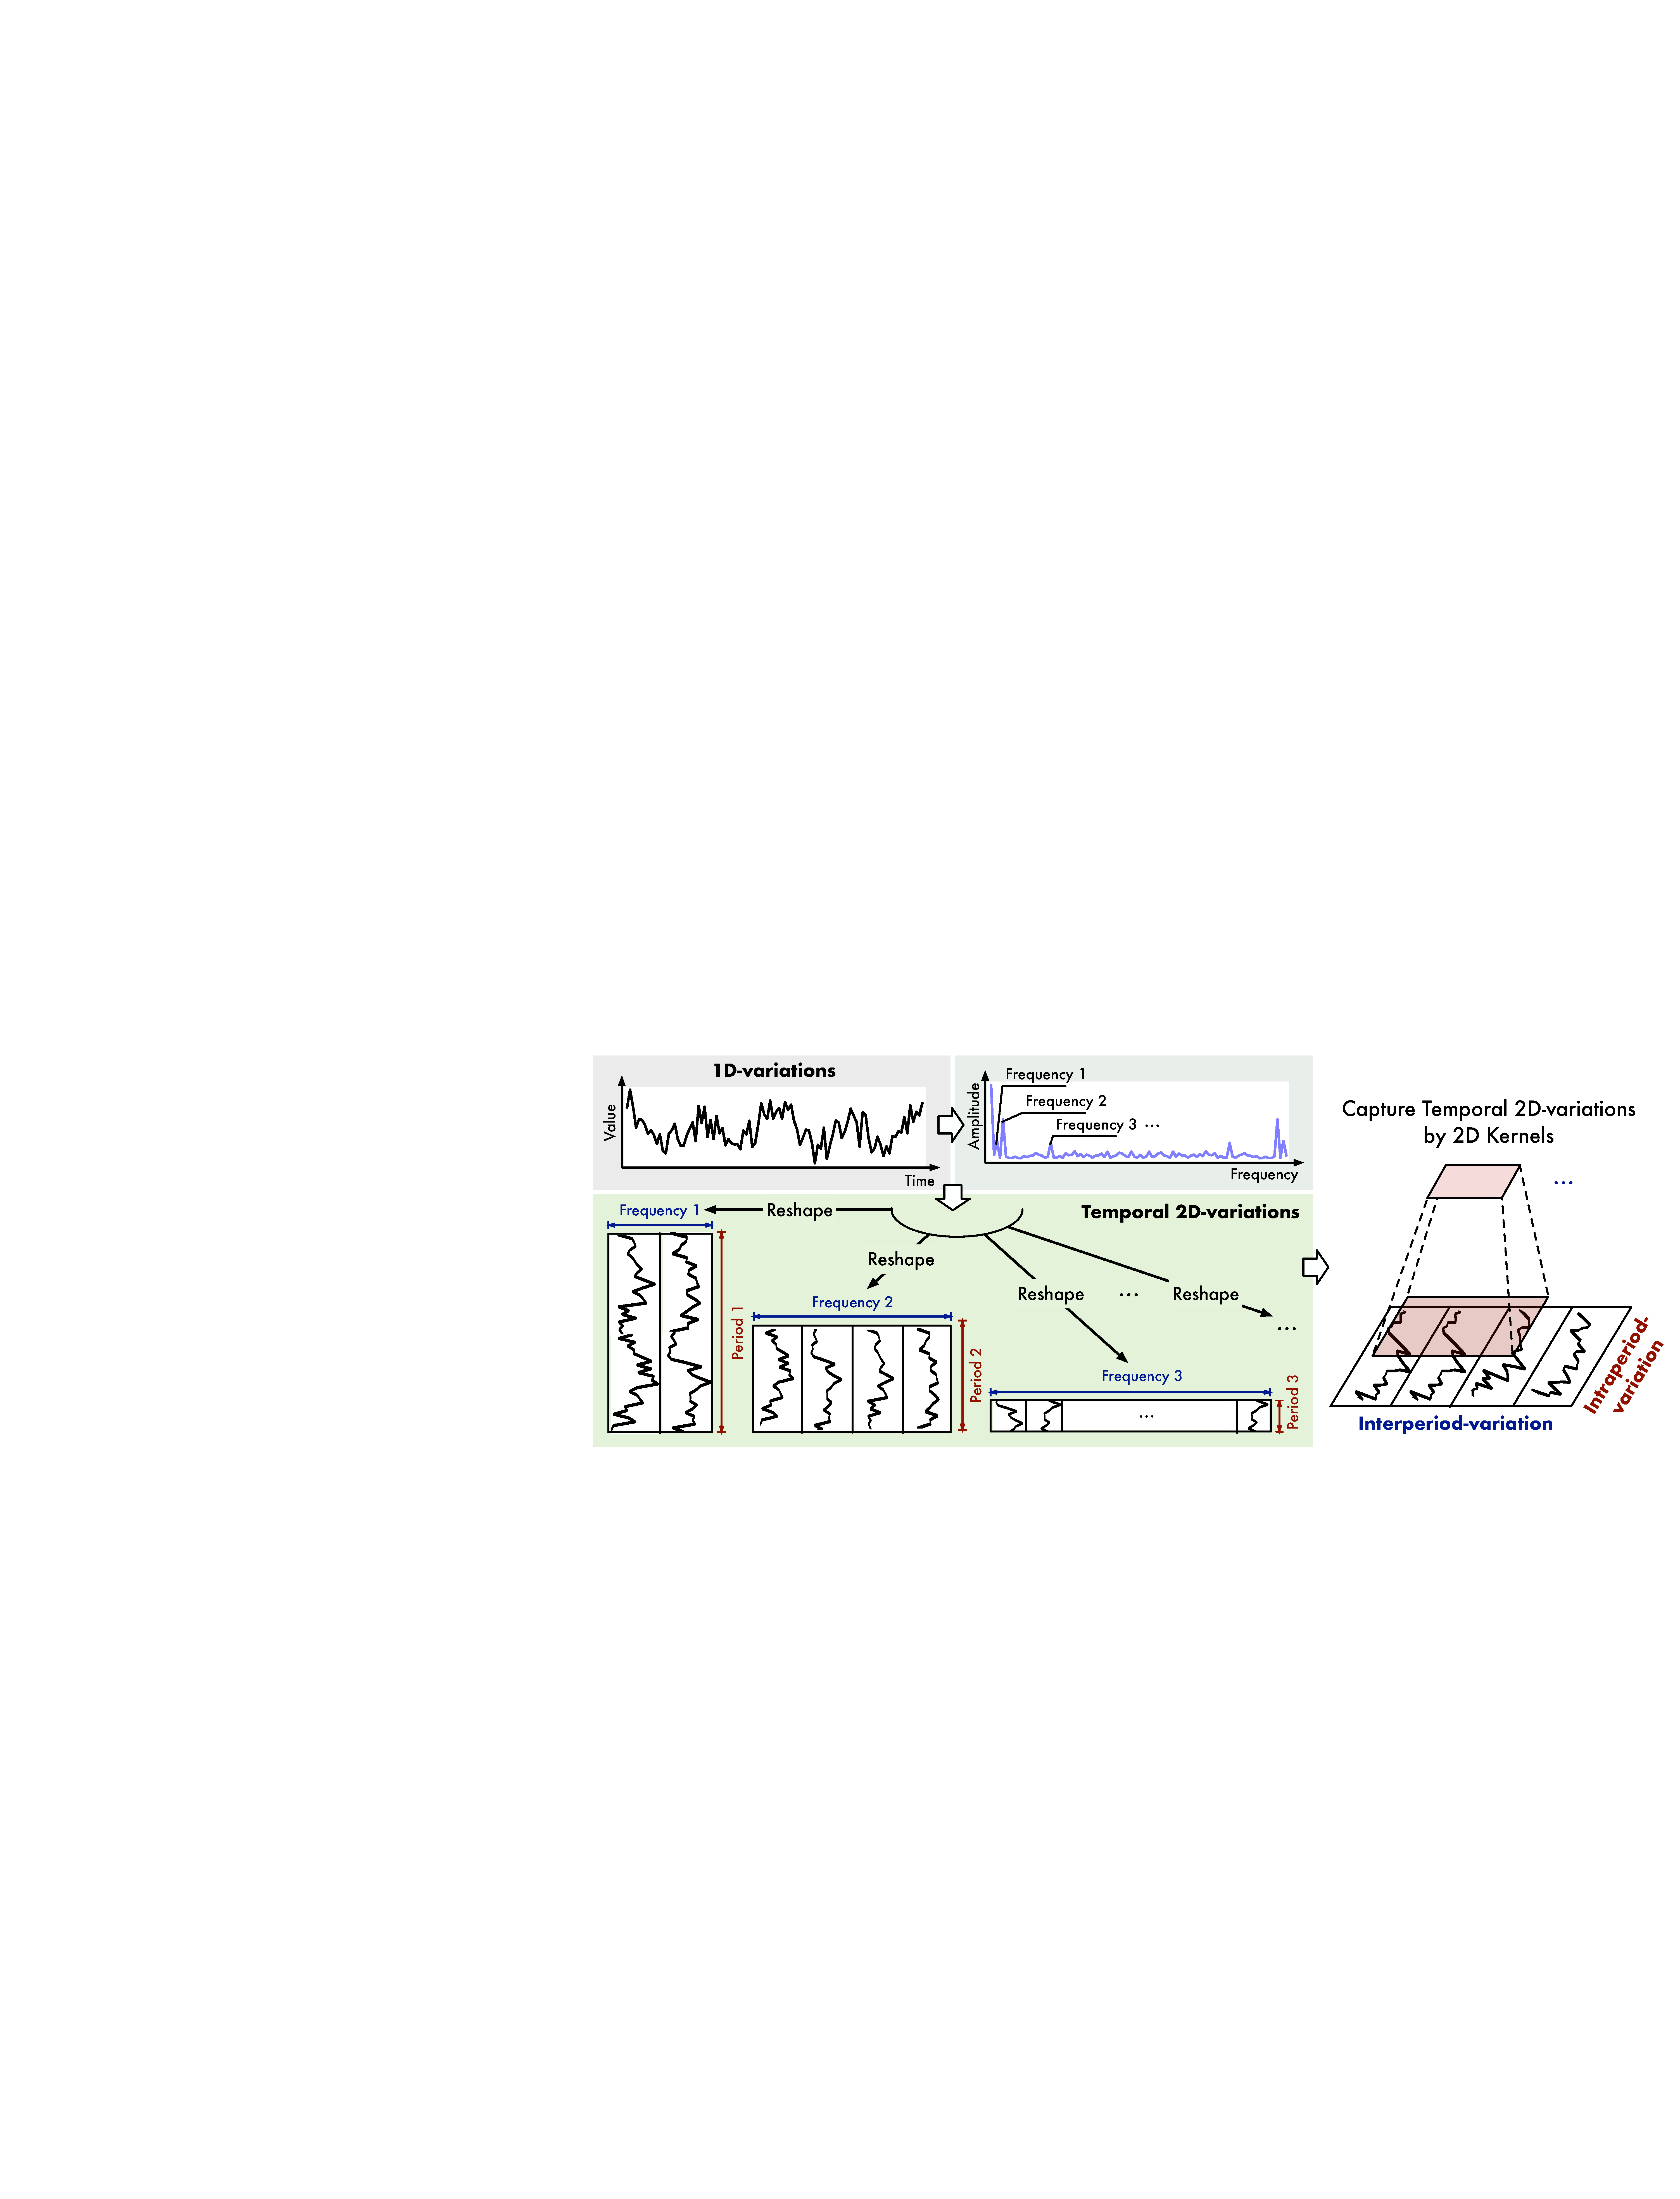
\includegraphics[width=1.0\textwidth]{imgs/timesnet_2d_structure.pdf}
    \caption{TimesNet 2D transformation: converting 1D time series into structured 2D tensors by discovering periodicity~\cite{wu_timesnet_2023}.}
    \label{fig:timesnet_2d_transformation}
\end{figure}

TimesNet shows better performance across four main time series analysis tasks: short-term and long-term forecasting, classification, and anomaly detection.

The model's ability to handle various sequence lengths and its strong design for capturing time dynamics work well with the requirements of battery degradation modeling, where both short-term changes and long-term trends must be considered at the same time. The key advantages include:

\begin{itemize}
\item \textbf{Multi-scale time modeling}: The 2D transformation allows capturing both short-term battery behavior (within periods) and long-term degradation trends (across periods) at the same time.
\item \textbf{Automatic period detection}: The FFT-based period discovery can identify natural cycles in battery operation without manual setup.
\item \textbf{Efficiency}: The shared inception block design keeps the model compact while handling multiple time scales.
\item \textbf{Flexibility}: The general-purpose nature allows adaptation to different battery types and operating conditions.
\end{itemize}

Unlike previous methods that struggle with the complex time patterns in battery data, TimesNet's 2D approach makes time changes easier to analyze. The transformation breaks the limitation of representation ability in the original 1D space, enabling more effective modeling of complex battery degradation patterns. The TimesNet architecture was therefore adapted for battery health prediction with several key modifications to optimize performance for this specific domain:

\begin{itemize}
    \item \textbf{Input preprocessing}: Battery measurement sequences were formatted. The input sequences were structured to capture both charge-discharge cycles and longer-term aging patterns.
    \item \textbf{Output configuration}: Modified for regression tasks to predict continuous SoH values rather than classification outputs. The final layer was adapted to output single scalar values representing battery health percentages.
    \item \textbf{Loss function}: Used MSE with additional rules to prevent overfitting and ensure stable training.
    \item \textbf{Feature engineering}: Minimal manual feature creation to use the model's automatic pattern discovery abilities. 
    \item \textbf{Period selection}: The top-k parameter was optimized specifically for battery data characteristics, allowing the model to focus on the most relevant repeating patterns in battery operation and degradation cycles.
\end{itemize}

\subsection{Hyperparameter Search}

For model optimization, the Optuna tool detailed in Section~\ref{subsec:optuna} was utilized, which enables hyperparameter optimization for machine learning models, integrated with WandB detailed in Section~\ref{subsec:wandb}, which allows for result visualization and model comparison. The dataset was reduced to only 1/10 of the data, equally distributed from the original dataset, with the objective of reducing the time required for finding the best hyperparameters, since this process took approximately one week even with this data reduction.

For the hyperparameter search, 50 trials were performed, with 50 epochs each, using an early stopping patience of 5 epochs to avoid overfitting and accelerate the optimization process. The parameters that were optimized through Optuna are:

\begin{itemize}
    \item \textbf{e\_layers}: Number of encoder layers (1--3) --- controls the depth of the encoder stack
    \item \textbf{d\_layers}: Number of decoder layers (1--3) --- controls the depth of the decoder stack  
    \item \textbf{factor}: Expansion factor for the FFN (1--5) --- controls the complexity of frequency components in TimesNet
    \item \textbf{freq}: Frequency for time features encoding (``s'', ``t'', ``h'') --- seconds, minutes, hours
    \item \textbf{d\_model}: Model dimension (fixed at 16)
    \item \textbf{top\_k}: Top-k dominant frequencies in TimesNet (1--5) --- controls how many frequency components to consider
\end{itemize}

Through this optimization, it was possible to detect the importance of the hyperparameters. The analysis showed that the importance factor of the \textbf{e\_layers} parameter (number of encoder layers) is the parameter that most influences the result when changed, demonstrating that the depth of the encoder architecture is critical for model performance. Figure~\ref{fig:hyperparameter_importance} illustrates the relative importance of each hyperparameter in the optimization process, clearly showing that \textbf{e\_layers} dominates with an importance score of 0.59, followed by \textbf{factor} (0.22) and \textbf{top\_k} (0.18).

\begin{figure}[htbp]
    \centering
    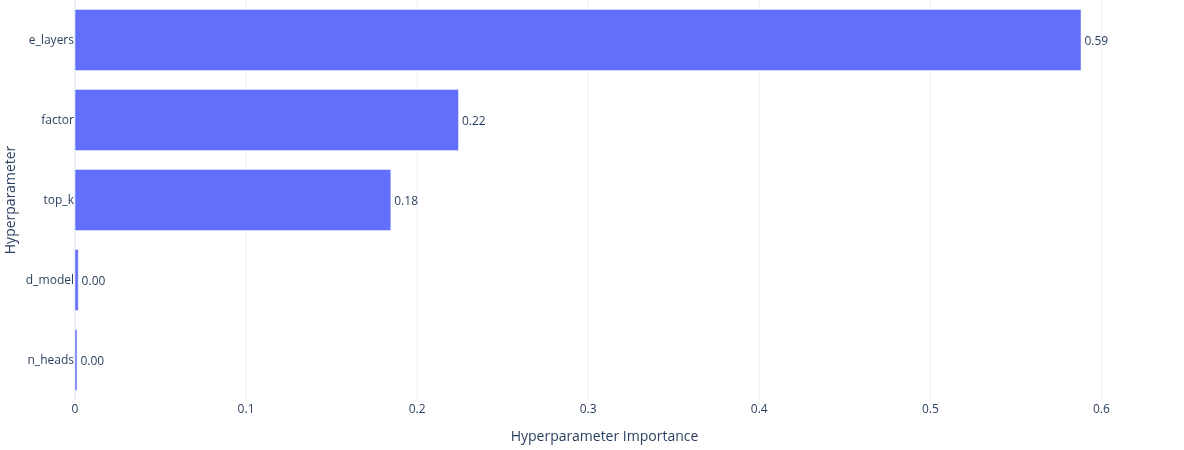
\includegraphics[width=1\textwidth]{imgs/Hyperparameter_importance.png}
    \caption{Hyperparameter importance analysis showing the relative influence of each parameter on model performance during Optuna optimization.}
    \label{fig:hyperparameter_importance}
\end{figure}

The hyperparameter optimization process can be further analyzed through the parallel coordinate plot shown in Figure~\ref{fig:parallel_coordinates}. This visualization technique displays the relationship between different hyperparameter configurations and their corresponding objective values (MSE loss). In the parallel coordinate plot, each vertical axis represents a different hyperparameter, and each line connects the parameter values for a single trial, with the line color indicating the objective value performance.

\begin{figure}[htbp]
    \centering
    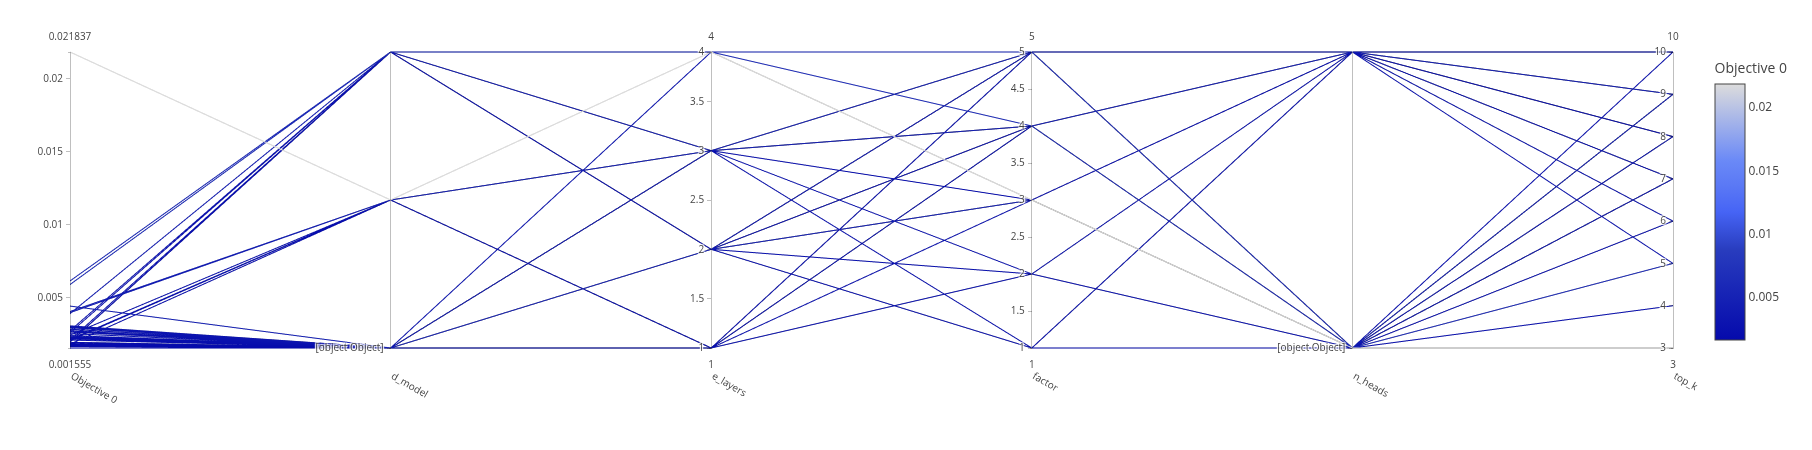
\includegraphics[width=1.0\textwidth]{imgs/objective_parallel_coordinate.png}
    \caption{Parallel coordinate plot showing the relationship between hyperparameter configurations and objective values across all 50 optimization trials. Each line represents a trial, with color intensity indicating performance (darker lines represent better MSE values).}
    \label{fig:parallel_coordinates}
\end{figure}

The parallel coordinate visualization reveals several important insights about the hyperparameter space:

\begin{itemize}
    \item \textbf{Convergence patterns}: The darker lines (representing trials with lower MSE values) show clustering around specific parameter combinations, indicating optimal regions in the hyperparameter space.
    \item \textbf{Parameter interactions}: The plot reveals how different parameter combinations interact with each other, particularly showing that successful trials tend to have \textbf{e\_layers} values of 2, which aligns with the importance analysis.
    \item \textbf{Search efficiency}: The distribution of lines across the parameter space demonstrates Optuna's efficient exploration strategy, focusing sampling on promising regions as the optimization progresses.
    \item \textbf{Trade-off visualization}: The varying line colors across different parameter combinations help identify trade-offs between different hyperparameter settings and their impact on model performance.
\end{itemize}

Additionally, Figure~\ref{fig:optuna_objective} shows the progression of the objective value throughout the optimization process, demonstrating how Optuna efficiently converges toward better solutions over the 50 trials.

\begin{figure}[htbp]
    \centering
    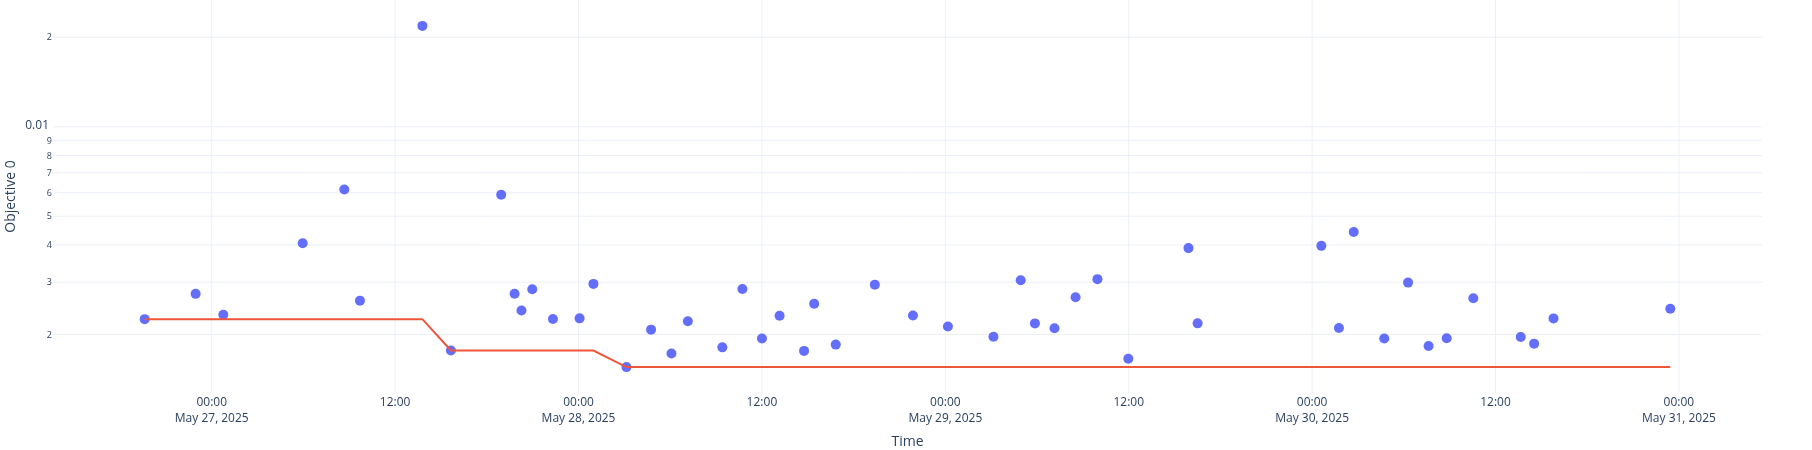
\includegraphics[width=1\textwidth]{imgs/optuna_objective_plot.png}
    \caption{Optuna objective value progression showing the improvement in MSE loss over 50 optimization trials.}
    \label{fig:optuna_objective}
\end{figure}

\textbf{Network Optimization Discussion}
\label{subsec:best_trial_results}

The most successful trial was trial 15, which presented the following results:

\begin{itemize}
    \item \textbf{MSE Value}: 0.0015545075293630362
    \item \textbf{Optimal Parameters}:
    \begin{itemize}
        \item e\_layers: 2
        \item factor: 4  
        \item d\_model: 16
        \item top\_k: 9
        \item n\_heads: 16
    \end{itemize}
    \item \textbf{Duration}: 7770232 ms (approximately 2 hours and 10 minutes)
\end{itemize}

The results show that using 2 encoder layers works better than deeper networks, likely avoiding overfitting on the battery dataset. The high expansion factor of 4 allows the model to capture more complex patterns, while setting top\_k to 9 means the model considers more frequency components than the default range, which helps capture the various periodic behaviors in battery degradation cycles.

The optimization process was also monitored using Weights \& Biases, which provided tracking of the validation loss across all trials. This monitoring proved extremely valuable for verifying that training was proceeding correctly, particularly given the very slow process of the hyperparameter search process. The ability to observe real-time training progress allowed for early detection of problematic configurations and ensured efficient use of computational resources during the time of optimization process. Figure~\ref{fig:wandb_validation_loss} shows the validation loss curves for different trials, illustrating the convergence behavior and helping identify the most promising hyperparameter configurations during the optimization process.

\begin{figure}[htbp]
    \centering
    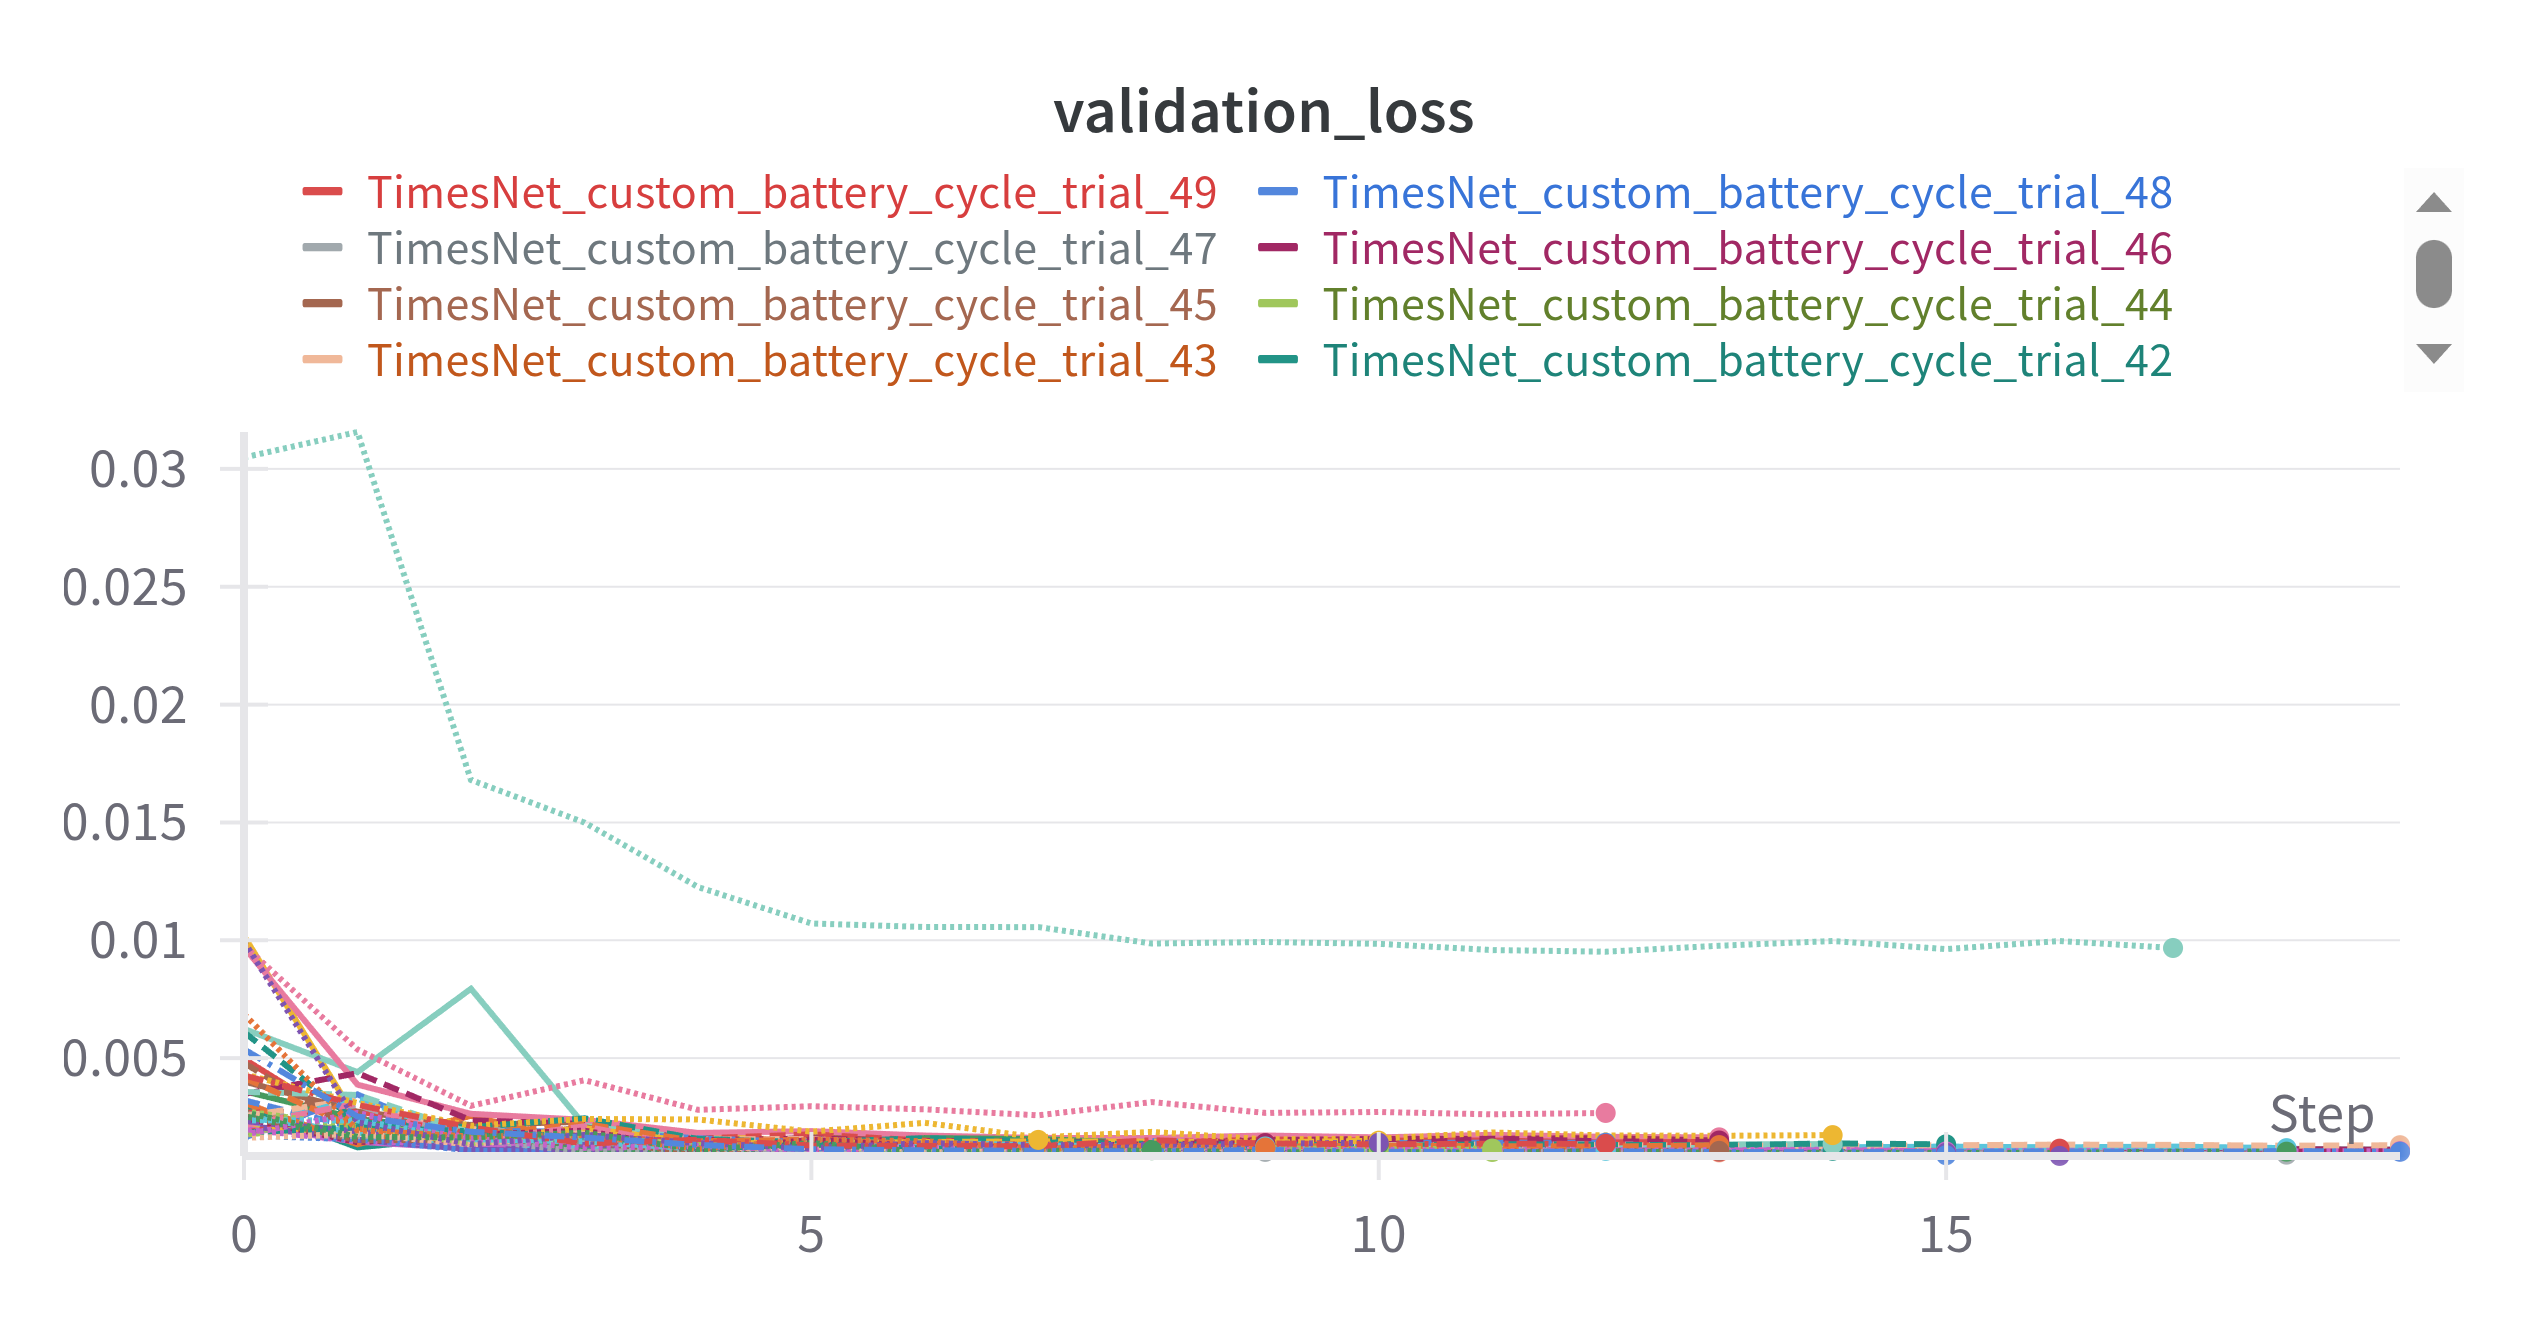
\includegraphics[width=1.0\textwidth]{imgs/W&B_optimization_validation_loss.png}
    \caption{Weights \& Biases validation loss tracking across multiple Optuna trials, showing the convergence behavior and performance comparison between different hyperparameter configurations.}
    \label{fig:wandb_validation_loss}
\end{figure}

\chapter{Experiments and Results}
\label{sec:experiments_results}

This chapter presents the comprehensive experimental evaluation of the TimesNet architecture for battery health prediction. The experiments were conducted using the optimized hyperparameters obtained from the Optuna search process detailed earlier. The model was trained to simultaneously predict SOC, SOH, and RUL from multi-dimensional battery operational data.

\section{Model Training Configuration}
\label{sec:training_config}

The TimesNet model was trained using the optimal hyperparameters identified through the systematic optimization process. The model architecture includes the following key specifications:

\subsection{Model Architecture and Complexity}
\label{subsec:model_complexity}

The final TimesNet model comprises 37,515,455 trainable parameters, making it a substantially complex deep learning architecture. To provide perspective on this complexity, this parameter count is comparable to smaller versions of modern language models, for context, GPT-2 Small (2019) contains 124 million parameters, making our model approximately 30\% of that size. This comparison helps illustrate the computational requirements for general users unfamiliar with neural network scales.

The model's memory footprint is 143.42 MB, which presents important considerations for deployment scenarios. While this size makes the model suitable for modern desktop and server environments, it poses challenges for edge device deployment. The memory requirements exceed typical constraints for embedded systems or mobile devices, limiting real-time battery monitoring applications in resource-constrained environments such as in embedded battery management systems.

\subsection{Input Feature Configuration}
\label{subsec:input_features}

The model processes six essential input features that capture the comprehensive operational state of battery systems:

\begin{itemize}
    \item \textbf{Voltage(V)}: Primary electrical characteristic indicating battery terminal voltage
    \item \textbf{Current(A)}: Charge and discharge current measurements
    \item \textbf{Time}: Temporal information for sequence modeling
    \item \textbf{SOC}: SOC feedback for multi-task learning
    \item \textbf{SOH}: SOH feedback for degradation tracking
    \item \textbf{RUL}: RUL feedback for predictive modeling
\end{itemize}

The selection of voltage and current as the primary input parameters was driven by their fundamental importance and practical accessibility in battery monitoring systems. These parameters represent the \textbf{most basic and straightforward measurements} that can be obtained from any battery system without requiring specialized or expensive instrumentation. Unlike more complex measurements such as impedance spectroscopy, temperature gradients, or electrochemical impedance, voltage and current can be acquired using \textbf{simple, cost-effective sensors} that are readily available in commercial battery management systems. This approach ensures that the developed model can be practically implemented in real world applications without requiring sophisticated measurement infrastructure, making it accessible for widespread deployment in various battery monitoring scenarios.

This multi-dimensional input configuration enables the model to learn complex interdependencies between different battery state variables, supporting the simultaneous prediction of multiple health indicators.

\subsection{Training Performance and Convergence}
\label{subsec:training_performance}

The model was trained for 43 epochs with a total training time of 39.81 hours. The training process demonstrated the following performance characteristics:

\begin{itemize}
    \item \textbf{Final Training Loss}: 0.07669
    \item \textbf{Final Validation Loss}: 0.02939
    \item \textbf{Final Test Loss}: 0.05030
    \item \textbf{Learning Rate}: 0.001 (fixed)
    \item \textbf{Batch Size}: 32
    \item \textbf{Total Training Steps}: 3,756
\end{itemize}

The training process utilized 120,169 samples for training, 4,900 samples for validation, and 4,910 samples for testing, ensuring robust evaluation across different data distributions.

\begin{figure}[htbp]
\centering
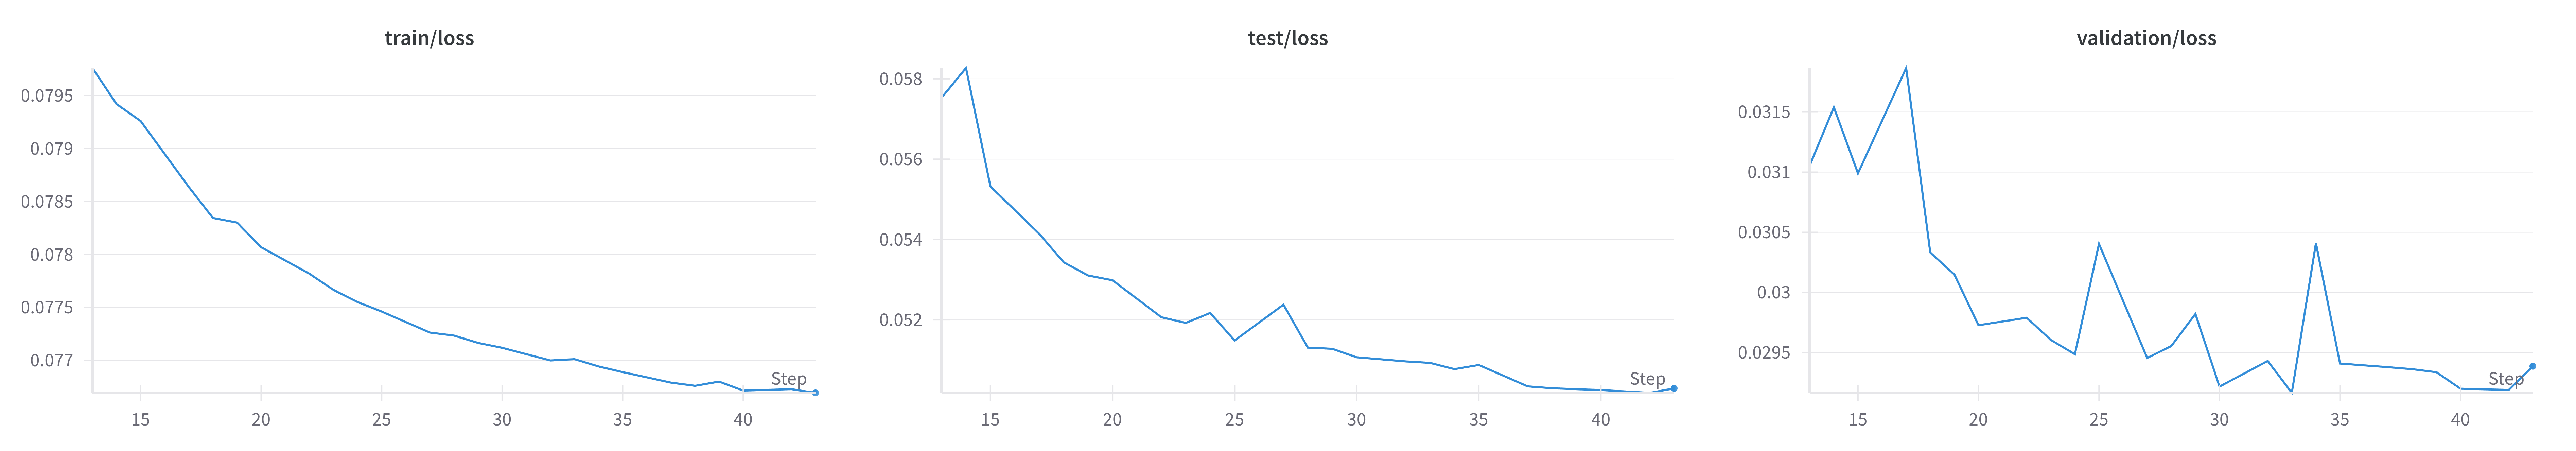
\includegraphics[width=1.0\textwidth]{imgs/loss_funtions.png}
\caption{Training, validation, and test loss progression throughout the training process, showing individual convergence behavior for each dataset split and demonstrating the generalization performance of the TimesNet model.}
\label{fig:training_losses}
\end{figure}

Figure~\ref{fig:training_losses} presents the training progression across all three dataset splits, with separate plots showing the individual loss curves for training, validation, and test sets. The plots illustrate the convergence behavior and demonstrate how the model performs across different data distributions throughout the optimization process.

\subsubsection{Training Convergence Analysis}
\label{subsubsec:training_convergence}

The training progression demonstrates several key characteristics that provide insights into model performance and learning stability:

\textbf{Positive Training Indicators}: The training loss exhibits a steady downward trend throughout the optimization process, indicating that the model is effectively learning patterns from the training data. The test loss also decreases consistently and remains below the training loss, suggesting good generalization capability without significant overfitting. The validation loss, despite exhibiting some fluctuation, reaches its lowest point at the end of training and shows no signs of divergence or instability, indicating stable learning progression.

\textbf{Areas of Concern}: The validation loss exhibits considerable noise throughout training, with frequent fluctuations that may indicate several potential issues. This variability could be attributed to the relatively small validation set size (4,900 samples), which increases variance in loss measurements. Additionally, the noisy validation curve may suggest that the model requires additional regularization or exhibits sensitivity to small changes in the validation data distribution.

\textbf{Training-Test Loss Relationship}: An unusual characteristic observed is that the test loss consistently performs better than the training loss throughout most of the training process. While this could indicate good generalization, it represents atypical behavior that warrants further investigation. This pattern may result from differences in how the metrics are computed across datasets or variations in data distribution between training and test sets.

The overall training behavior suggests a stable learning process with good convergence properties, though the validation loss volatility indicates potential areas for improvement in model regularization and training stability.

\section{Model Testing and Performance Evaluation}
\label{sec:model_testing}

The trained TimesNet model was evaluated separately for each target variable (SOC, SOH, and RUL) to assess its performance in multi-task battery health prediction. The evaluation provides comprehensive performance metrics across different battery health indicators.

\subsection{SOC Prediction Results}
\label{subsec:soc_results}

The SOC prediction performance demonstrates the model's capability to track charge state variations within battery operational cycles. Table~\ref{tab:soc_results} presents the comprehensive evaluation metrics for SOC estimation.

\begin{table}[htbp]
\centering
\caption{SOC prediction performance metrics}
\label{tab:soc_results}
\begin{tabular}{lc}
\hline
\textbf{Metric} & \textbf{Value} \\
\hline
MAE & 0.0621 \\
MSE & 0.0507 \\
RMSE & 0.2251 \\
\hline
\end{tabular}
\end{table}

The SOC results show strong performance with a relatively low RMSE of 0.2251, demonstrating accurate tracking of charge state variations.

%\begin{figure}[htbp]
%\centering
%\includegraphics[width=1.0\textwidth]{imgs/soc_comprehensive_analysis.png}
%\caption{Comprehensive SOC prediction analysis showing prediction accuracy, error distribution, and time series comparison between predicted and actual SOC values.}
%\label{fig:soc_analysis}
%\end{figure}

\subsection{SOH Prediction Results}
\label{subsec:soh_results}

The SOH prediction results reveal the challenges associated with modeling battery degradation patterns. Table~\ref{tab:soh_results} presents the performance metrics for SOH estimation.

\begin{table}[htbp]
\centering
\caption{SOH prediction performance metrics}
\label{tab:soh_results}
\begin{tabular}{lc}
\hline
\textbf{Metric} & \textbf{Value} \\
\hline
MAE & 0.2039 \\
MSE & 0.2790 \\
RMSE & 0.5282 \\
\hline
\end{tabular}
\end{table}

The SOH results show moderate performance with an RMSE of 0.5282, reflecting the increased difficulty in modeling long-term degradation patterns compared to SOC.

%\begin{figure}[htbp]
%\centering
%\includegraphics[width=1.0\textwidth]{imgs/soh_comprehensive_analysis.png}
%\caption{Comprehensive SOH prediction analysis showing prediction accuracy, error distribution, and time series comparison between predicted and actual SOH values.}
%\label{fig:soh_analysis}
%\end{figure}

\subsection{RUL Prediction Results}
\label{subsec:rul_results}

The RUL prediction represents the most challenging aspect of battery health modeling, as it requires accurate forecasting of future battery degradation. Table~\ref{tab:rul_results} presents the performance metrics for RUL estimation.

\begin{table}[htbp]
\centering
\caption{RUL prediction performance metrics}
\label{tab:rul_results}
\begin{tabular}{lc}
\hline
\textbf{Metric} & \textbf{Value} \\
\hline
MAE & 0.2078 \\
MSE & 0.2821 \\
RMSE & 0.5311 \\
\hline
\end{tabular}
\end{table}

The RUL results show the highest prediction errors among the three target variables, with an RMSE of 0.5311. This reflects the inherent complexity of predicting future battery life based on current operational patterns.

\section{Results Analysis and Discussion}
\label{sec:results_discussion}

The experimental results reveal important insights about the challenges and limitations of multi-task learning for battery health prediction using state-of-the-art deep learning architectures.

\subsection{Performance Analysis}
\label{subsec:performance_analysis}

The results demonstrate a clear performance hierarchy across the three prediction tasks:

\begin{enumerate}
    \item \textbf{SOC Prediction}: Achieved the best performance (RMSE = 0.2251)
    \item \textbf{SOH Prediction}: Showed moderate performance (RMSE = 0.5282)
    \item \textbf{RUL Prediction}: Exhibited the most challenging results (RMSE = 0.5311)
\end{enumerate}

This performance gradient reflects the increasing complexity of the prediction tasks. SOC prediction benefits from direct correlation with immediate electrical measurements, while SOH and RUL require modeling of long-term degradation patterns that are more difficult to capture accurately.

\subsection{Limitations and Challenges}
\label{subsec:limitations}

Despite utilizing a state-of-the-art TimesNet architecture, the results did not achieve the expected performance levels for multi-task battery health prediction. The \textbf{multi-task learning complexity} presents the most significant challenge, as simultaneous prediction of SOC, SOH, and RUL in a single network creates \textbf{competing optimization objectives}. Each target variable has fundamentally different temporal characteristics - SOC prediction benefits from short-term electrical patterns, while SOH and RUL require long-term degradation modeling. This creates \textbf{conflicting gradients} during training that limit overall performance.

Additionally, the \textbf{multi-task approach prevents architectural specialization}, meaning the network cannot focus entirely on the specific patterns most relevant to each individual prediction task. While TimesNet provides advanced temporal modeling capabilities, the shared architecture must balance between three different objectives rather than excelling at one. This trade-off between \textbf{system integration} and \textbf{individual task performance} represents a fundamental limitation of the unified approach.

\subsection{Comparison with Simpler Approaches}
\label{subsec:comparison_simpler}

When comparing these results with simpler neural network approaches that focus on single-task prediction (e.g., networks designed exclusively for SOC estimation), the trade-offs become apparent. Single-task networks typically achieve better performance on their specific target due to their \textbf{specialized architecture}, where the entire network capacity is dedicated to one prediction task. This allows for \textbf{focused optimization}, as training optimization is not diluted across multiple objectives, and enables \textbf{task-specific features} where feature extraction can be optimized for the specific characteristics of the target variable.

The multi-task approach, while providing comprehensive battery health monitoring in a single model, sacrifices individual task performance for \textbf{system integration} and \textbf{computational efficiency}. This represents a fundamental trade-off in deep learning system design between specialized performance and unified functionality.



\chapter{Conclusion and Future Work}
\label{sec:conclusion_future_work}

This chapter presents the key findings, achievements, and limitations of the BattAIHealth project, along with recommendations for future research directions. The project represents a comprehensive exploration of battery health prediction using state-of-the-art deep learning techniques, spanning from traditional MATLAB-based approaches to cutting-edge TimesNet architectures for simultaneous prediction of SOC, SOH, and RUL.

\section{Conclusion}
\label{sec:conclusion}

This project was exceptionally challenging and extended far beyond the typical scope of coursework. It required deep exploration of advanced concepts and technologies that I had never encountered before, providing invaluable learning experiences with tools and methodologies that will undoubtedly prove essential for future professional projects.

The journey through this project encompassed multiple phases of technological exploration. I started with traditional MATLAB-based modeling using Extended Kalman Filters and physics-based Batemo battery models, then explored hybrid CNN-LSTM architectures, investigated cutting-edge Transformer and Mixture of Experts networks, and ultimately implemented the state-of-the-art TimesNet architecture for multi-task battery health prediction. Each phase taught me something new and highlighted just how complex accurate battery health monitoring really is.

Working with the MATLAB implementation taught me the fundamentals of traditional battery modeling techniques. The Extended Kalman Filters and physics-based simulation using the Batemo INR21700-p45b model provided crucial insights into the challenges of battery state estimation and the limitations of conventional approaches. This foundation was essential for understanding why more advanced approaches were needed.

The exploration of neural network architectures revealed important trade-offs between model complexity and performance. The comparative analysis between Transformer and Mixture of Experts networks was particularly interesting - I discovered that simpler architectures can achieve competitive performance with significantly reduced computational requirements. The MoE implementation achieved an RMSE of 0.0335 compared to the Transformer's 0.0297, representing a minimal performance difference while offering substantial computational advantages.

The TimesNet implementation was the most technically challenging part of the project. It required mastering advanced concepts including FFT-based period detection, 2D transformation of time series data, and multi-task learning optimization. The systematic hyperparameter optimization using Optuna across 50 trials with 50 epochs each was a rigorous process that highlighted the critical importance of encoder depth in model performance.

However, the results were not as good as I initially hoped. The TimesNet model achieved differentiated performance across the three prediction tasks, with SOC prediction showing the best results (RMSE = 0.2251), followed by SOH (RMSE = 0.5282) and RUL (RMSE = 0.5311) prediction. While this represents a substantial engineering achievement, it did not reach the initially anticipated performance levels for multi-task learning.

The project taught me that general-purpose solutions, while appealing for their comprehensiveness, may not always be the optimal approach for specific problems. The multi-task learning approach, despite using a state-of-the-art TimesNet architecture, highlighted the fundamental trade-off between system integration and individual task performance. This suggests that specialized architectures optimized for specific prediction tasks may achieve superior performance compared to unified approaches.

The computational complexity of the final model (37.5 million parameters, 143.42 MB memory footprint) also presents practical deployment challenges, particularly for resource-constrained embedded systems typical in automotive and railway applications. The hyperparameter optimization process required approximately one week of computational time even with reduced dataset size, highlighting the substantial computational resources required for comprehensive model optimization.

Despite these limitations, this type of research carries significant practical importance as the world continues its transition toward electrification. The increasing adoption of electric vehicles, renewable energy storage systems, and battery-powered industrial equipment creates growing demand for accurate, reliable battery health monitoring solutions. The extreme operating conditions in automotive and railway applications—including temperature variations, vibrations, and demanding load profiles—make battery health prediction particularly challenging and important for safety and reliability.

\section{Future Work}
\label{sec:future_work}

Based on the findings from this project, several promising directions emerge for future research and development in battery health prediction systems. The main lesson learned is that trying to solve all three prediction tasks (SOC, SOH, and RUL) simultaneously may not be the best approach for achieving optimal individual task performance.

The analysis of the multi-task learning approach revealed fundamental limitations that point toward more effective alternative strategies. The competing optimization objectives between SOC, SOH, and RUL prediction create conflicting gradients during training, while the shared architecture prevents the specialization needed for each distinct prediction task. These insights suggest that future research should focus on approaches that leverage task-specific architectures while maintaining the benefits of comprehensive battery health monitoring.

The most promising direction for future work involves developing ensemble methods that combine multiple specialized models, each optimized for individual prediction tasks~\cite{noauthor_pdf_nodate}. Rather than forcing one large model to handle everything, this approach would deploy separate models strategically designed for their specific purposes: CNNs for feature extraction from voltage and current profiles in SOC estimation, LSTM networks specifically engineered for time-series RUL prediction, and gradient-boosted decision trees for SOH estimation. These specialized models could then be integrated using advanced fusion techniques such as weighted averaging, stacking methods, or boosting approaches, allowing each component to excel in its domain while maintaining comprehensive monitoring capabilities.

Transfer learning and sequential task modeling present another compelling direction that could address the task interdependency challenges observed in this work~\cite{zhuang_comprehensive_2021}. This hierarchical approach would exploit the natural dependencies between battery health indicators by pre-training models on abundant SOC data and subsequently fine-tuning for SOH and RUL prediction. The sequential modeling paradigm, where SOC predictions feed into SOH estimation and both inform RUL prediction, would explicitly model the causal relationships between these variables while avoiding the competing optimization objectives that limited the unified approach.

The integration of physics-based knowledge through physics-informed neural networks offers significant opportunities for improving both model performance and interpretability~\cite{raissi_physics-informed_2019}. This hybrid approach would combine electrochemical models, such as Thevenin equivalent circuits for SOC estimation, with data-driven models for capturing complex degradation patterns in SOH and RUL prediction. The physics-informed approach could provide regularization for neural network training while ensuring that predictions respect fundamental battery physics principles, potentially leading to more robust and trustworthy predictions.

Advanced graph neural networks represent another innovative direction where battery data is represented as graphs to capture complex temporal and electrochemical relationships~\cite{zhou_graph_2020}. In this framework, nodes would represent battery measurements at different time steps, while edges would encode temporal dependencies and physical relationships. This approach could be particularly valuable for battery pack applications where cell-to-cell interactions significantly influence overall system health, extending beyond single-cell prediction to comprehensive system-level monitoring.

The practical deployment challenges identified in this work require dedicated attention in future research. Developing efficient model architectures specifically designed for real-time deployment in resource-constrained environments remains a critical need. This includes exploring model compression techniques, knowledge distillation approaches, and hardware-aware neural architecture search methods to create edge-optimized models that can run efficiently on embedded systems typical in automotive and railway applications.